\documentclass[10pt, proquest]{uwthesis}[2014/11/13]

\setcounter{tocdepth}{1}

\usepackage{amsmath}
\usepackage{amsfonts}
\usepackage{amsthm}
\usepackage{amssymb}
\usepackage{graphicx}
\usepackage[font={small,it}]{caption}
\usepackage{subcaption}
\usepackage{color}
\usepackage[section]{algorithm}
\usepackage{algpseudocode}
\usepackage{tikz}
\usetikzlibrary{shapes,matrix,arrows,decorations,decorations.markings,tikzmark,fit,shapes.geometric,decorations.pathmorphing,backgrounds,positioning}

\usepackage{url}
\usepackage{hyperref}
\def\chapterautorefname{Chapter}
\def\sectionautorefname{Section}
\usepackage{listings}
\usepackage[T1]{fontenc}
\usepackage{inconsolata}
\lstdefinelanguage{Sage}[]{Python}
{morekeywords={sage},
sensitive=true}
\lstset{frame=none,
        showtabs=False,
        showspaces=False,
        showstringspaces=False,
        commentstyle={\it\ttfamily\color{gray}},
        keywordstyle={\bf\ttfamily\color{black}},
        stringstyle ={\ttfamily\color{gray}},
        language=Sage,
        basicstyle={\footnotesize\ttfamily},
        xleftmargin=1em,
        aboveskip=1em,
        belowskip=1em,
        upquote=true
      }

% the quotation environment is used for section summaries
\usepackage{etoolbox}
\AtBeginEnvironment{quote}{\footnotesize}

\usepackage{enumitem}
\setlist[1]{itemsep=-5pt}

\newtheorem{theorem}[algorithm]{Theorem}
\newtheorem{proposition}[algorithm]{Proposition}
\newtheorem{lemma}[algorithm]{Lemma}
\newtheorem{corollary}[algorithm]{Corollary}
\newtheorem{definition}[algorithm]{Definition}
\theoremstyle{definition}
\newtheorem{example}[algorithm]{Example}
\numberwithin{equation}{section}

\newcommand{\secondkind}[2]{\omega_{#1}^{(#2)}}
\newcommand{\dd}{\,\mathrm{d}}
\newcommand{\dx}{\,\mathrm{d}x}
\newcommand{\dt}{\,\mathrm{d}t}
\newcommand{\dP}{\,\mathrm{d}P}
\newcommand{\dQ}{\,\mathrm{d}Q}
\newcommand{\PP}[1]{\mathrm{P}^#1 \!}
\DeclareMathOperator{\re}{\text{Re}}
\DeclareMathOperator{\im}{\text{Im}}
\DeclareMathOperator{\ZZ}{\mathbb{Z}}
\DeclareMathOperator{\RR}{\mathbb{R}}
\DeclareMathOperator{\CC}{\mathbb{C}}
\DeclareMathOperator{\hh}{\mathfrak{h}}
\DeclareMathOperator{\hg}{\mathfrak{h}_g}
\DeclareMathOperator{\DivC}{\mathcal{C}}
\DeclareMathOperator{\DivD}{\mathcal{D}}
\DeclareMathOperator{\RCV}{\boldsymbol{K}}
\DeclareMathOperator{\Abel}{\boldsymbol{A}}
\DeclareMathOperator{\HalfLattice}{\Lambda_{1/2}}

\newcommand{\thchar}[2] {\begin{bmatrix}#1\\#2\end{bmatrix}}
\newcommand{\thcharsm}[2] {\left[ \begin{smallmatrix} #1
      \\ #2 \end{smallmatrix} \right]}

\title{Ph.D. Thesis}
\author{Chris Swierczewski}
\date{\today}

%%%%%%%%%%%%%%%%%%%%%%%%%%%%%%%%%%%%%%%%%%%%%%%%%%%%%%%%%%%%%%%%%%%%%%%%%%%%%%%
\begin{document}
%%%%%%%%%%%%%%%%%%%%%%%%%%%%%%%%%%%%%%%%%%%%%%%%%%%%%%%%%%%%%%%%%%%%%%%%%%%%%%%

% preliminary pages
%
\prelimpages
%\include{prelim}

\clearpage
\thispagestyle{empty}
\vspace*{\fill}
\begin{quote}
  \center
  \em The standard of correctness and completeness necessary to get a computer
  program to work at all is a couple of orders of magnitude higher than the
  mathematical community's standard of valid proofs. Nonetheless, large
  computer programs, even when they have been very carefully written and very
  carefully tested, always seem to have bugs.
  \center
  \medskip
  \raggedleft
  \medskip
  --- William P. Thurston
\end{quote}
\vspace*{\fill}

% text pages
%
\textpages
%%%%%%%%%%%%%%%%%%%%%%%%%%%%%%%%%%%%%%%%%%%%%%%%%%%%%%%%%%%%%%%%%%%%%%%%%%%%%%%
\chapter{Introduction}
%%%%%%%%%%%%%%%%%%%%%%%%%%%%%%%%%%%%%%%%%%%%%%%%%%%%%%%%%%%%%%%%%%%%%%%%%%%%%%%


%%%%%%%%%%%%%%%%%%%%%%%%%%%%%%%%%%%%%%%%%%%%%%%%%%%%%%%%%%%%%%%%%%%%%%%%%%%%%%%
\chapter{Complex Algebraic Geometry and Riemann Surfaces}\label{ch:background}
%%%%%%%%%%%%%%%%%%%%%%%%%%%%%%%%%%%%%%%%%%%%%%%%%%%%%%%%%%%%%%%%%%%%%%%%%%%%%%%

In this chapter we will give a brief overview of Riemann surfaces from the
perspective of complex algebraic geometry. Among the primary references used in
this thesis, Griffiths \cite{Giffiths89} provides one of the most succinct
introductions to the subject without requiring background in algebraic geometry
or algebraic curves and gives solid foundation from which to further explore the
topic. Ueno's \cite{Ueno97} presentation is similar but with more emphasis on
the algebraic perspectives whereas Bliss \cite{bliss} focuses on an analytic
approach, instead. Dubrovin's \cite{Dubrovin81} classical manuscript includes
connections to the Kadomtsev-Petviashvili equation introduced in
\autoref{ch:kp}.

%%%%%%%%%%%%%%%%%%%%%%%%%%%%%%%%%%%%%%%%%%%%%%%%%%%%%%%%%%%%%%%%%%%%%%%%%%%%%%%
\section{Complex Algebraic Geometry}\label{sec:background-complex-algebraic-geometry}
%%%%%%%%%%%%%%%%%%%%%%%%%%%%%%%%%%%%%%%%%%%%%%%%%%%%%%%%%%%%%%%%%%%%%%%%%%%%%%%

We begin with some preliminary constructions and facts from complex algebraic
geometry. This section culminates in the Normalization Theorem which connects
the subject to the study of Riemann surfaces. Although other computational
approaches to Riemann surfaces exist, this connection makes the computational
approach possible later.

%..............................................................................
\subsection{The Projective Line}
%..............................................................................

The primary motivation behind complex projective geometry is to make concrete
the way in which we analyze the behavior of functions, such as polynomials, at
infinity without having to resort to techniques separate from those used at
finite points. For example, in applications we may need to integrate a
differential along a path on an algebraic curve going to infinity. Knowing the
geometry of the curve at infinity makes such an operation computationally
feasible.

In fact, anyone with an elementary complex analysis background has seen an
example of projective geometry. The Riemann sphere is the complex plane $\CC$
with a ``point at infinity'' added. Let $z$ denote the coordinate in $\CC$
(i.e., the point $z=0$ represents the origin of the complex plane). In order to
discuss the point at infinity we introduce the coordinate $w = 1/z$. The
analysis of some function at $\infty$ is equivalent to rewriting the problem in
terms of the coordinate $w$ and examining its behavior in a neighborhood of
$w=0$. This explains why, for example, the exponential function
\[
  e^z = \sum_{n=0}^\infty z^n / n!,
\]
though entire in the complex plane, has an essential singularity on the Riemann
sphere since the exponential function in the coordinate $w$ centered at $w=0$ is
expressed by the series
\[
  \sum_{n=0}^\infty \frac{w^{-n}}{n!}.
\]

This point at infinity is not rigorously defined because it does not make sense
to {\it equate} $z=\infty$. The definition of the Riemann sphere is made
explicit by the following construction: consider the set $U = \CC^2 -
\{(0,0)\}$. Define the equivalence relation
\[
  (a_0, a_1) \sim (\lambda a_0, \lambda a_1), \quad \forall \lambda \in \CC -
  \{0\}.
\]
Thus two points $(a_0,a_1)$ and $(b_0,b_1)$ in $U$ are considered the same if
the ratios $a_0 : a_1$ and $b_0 : b_1$ are equal. The set of all points
$(b_0,b_1)$ equal to $(a_0,a_1)$ is called the {\it equivalence class} of
$(a_0,a_1)$ and the {\it complex projective line} $\PP{1}\CC$ is the set of all
such equivalence classes. That is,
\[
  \PP{1}\CC := \CC^2 / \sim.
\]
The equivalence class of $(a_0,a_1)$, called a ``point'' in $\PP{1}\CC$, is
written $(a_0 : a_1) \in \PP{1}\CC$. $\PP{1}\CC$ is precisely the Riemann
sphere. To see this, consider the two subsets
\begin{align*}
  U_0 &= \{ (a_0 : a_1) \in \PP{1}\CC \; | \; a_0 \neq 0 \}, \\
  U_1 &= \{ (a_0 : a_1) \in \PP{1}\CC \; | \; a_1 \neq 0 \}.
\end{align*}
For any $(a_0 : a_1) \in U_0$ we have, by the equivalence property,
\[
  (a_0 : a_1) = (1 : a_1/a_0) = (1 : a).
\]
Similarly, $(b_0 : b_1) = (b : 1)$ for every point in $U_1$. Every point in the
intersection $U_0 \cap U_1$ can be written in either of these two forms. Each of
these subspaces are isomorphic to $\CC$ since the maps
\begin{align*}
  \phi_0 : U_0 \to \CC,
  \quad
  \phi_0 \left( (a_0 : a_1) \right) = a_1 / a_0,
  & \quad \text{ and } \\
  \phi_1 : U_1 \to \CC,
  \quad
  \phi_1 \left( (a_0 : a_1) \right) = a_0 / a_1, &
\end{align*}
are continuous bijections with inverses
\begin{gather}
  \phi^{-1}_0(a) = (1 : a), \\
  \phi^{-1}_1(b) = (b : 1).
\end{gather}
Finally, note that $(0 : 1)$ is the only projective point in $U_1$ which is not
in $U_0$. Therefore, we identify $U_0$ with the complex plane (in the coordinate
$z$) and the point $P_\infty = (0 : 1)$ with the point at infinity and set
\begin{equation} \label{eqn: projective-line}
  \PP{1}\CC = U_0 \cup \{ (0 : 1) \} \cong \CC \cup P_\infty.
\end{equation}

Indeed $P_\infty$ is considered the point at infinity on the Riemann sphere for
if one considers the image of $(0 : 1)$ under $\phi_0$, though undefined since
$(0:1) \not \in U_0$, it maps to $z = 1 / 0$ ``='' $\infty$. Again, this does
not make sense without the complex projective space construction above but is
merely used to illustrate the point. The coordinate transformation from $z$ to
$w$ at the beginning of this section is equivalent to identifying $U_1$ with the
complex plane $\CC$ and $\{(1 : 0)\}$ with the point at infinity, instead.

%------------------------------------------------------------------------------
\subsection{The Projective Plane} \label{sec:projective-plane}
%------------------------------------------------------------------------------

The natural environment we use in the sequel is not the complex projective line
but the complex projective plane. In this section we construct the projective
plane and examine its geometric properties. The construction is similar to that
of the projective line.

Let $U = \CC^3 - \{(0,0,0)\}$. Following the strategy of the previous section,
consider the set of all ratios $(a_0 : a_1 : a_2)$, that is, the collection of
all equivalence classes under the equivalence relation $(a_0 : a_1 : a_2) \sim
(\lambda a_0 : \lambda a_1 : \lambda a_2), \forall \lambda \in \CC - \{0\}$. The
space of all such equivalence classes is called the two-dimensional complex
projective space or {\it the projective plane} and is denoted $\PP{2}\CC$.

Define the subsets $U_0,U_1,U_2$ by
\[
  U_j = \{ (a_0 : a_1 : a_2) \in \PP{2}\CC \; | \; a_j \neq 0 \},
\]
and note that all $(a_0 : a_1 : a_2) \in U_0$ satisfy $(a_0 : a_1 : a_2) = (1 :
a_1/a_0 : a_2/a_0)$. We define the bijective mapping
\begin{gather*}
  \phi_0 : U_0 \to \CC^2, \\
  \phi_0 \left( (a_0 : a_1 : a_2) \right) =
  \left( \frac{a_1}{a_0}, \frac{a_2}{a_0} \right), \\
  \phi_0^{-1} \left( (x,y) \right) = (1 : x : y).
\end{gather*}
The mappings $\phi_1$ and $\phi_2$ are similarly defined on $U_1$ and $U_2$,
respectively. Therefore, we can identify $U_0$ with the complex plane $\CC^2$.

Consider the space $U_0^c = \PP{2}\CC - U_0$. By definition, every point in
$U_0^c$ is of the form $(0 : a_1 : a_2)$. By definition, every point in $U_0^c$
determines a point on the complex projective line $\PP{1}\CC$. The converse is
true as well, resulting in the bijection
\[
  (0 : a_1 : a_2) \in \PP{2}\CC \; \leftrightarrow \; (a_1 : a_2) \in \PP{1}\CC.
\]
By identifying $U_0^c$ with $\PP{1}\CC$ we may write
\begin{equation} \label{eqn: proejctive-plane} \PP{2}\CC = U_0 \cup U_0^c \cong
  \CC^2 \cup \PP{1}\CC
\end{equation}
where $U_0^c \cong \PP{1}\CC$ is called the {\it line at infinity}, denoted
$l_\infty$, and $U_0 \cong \CC^2$ is called the {\it complex affine plane}. We
may also identify the complex affine plane with the sets $U_1$ or $U_2$ and the
line at infinity with their complements.

We saw a natural geometric interpretation of $\PP{1}\CC$ in the previous
section. Does such an interpretation exist for $\PP{2}\CC$? Consider a line in
the complex affine plane $\CC^2$ which can be written in the form
\[
  \alpha + \beta x + \gamma y = 0, \quad \text{where } (\beta,\gamma) \neq 0,
  \alpha, \beta, \gamma \in \CC.
\]
Using the inverse mapping $\phi_0^{-1}$ on $\CC^2$ we have
\[
  x = \frac{x_1}{x_0} \text{ and } y = \frac{x_2}{x_0},
\]
where $(x_0 : x_1 : x_2)$ are the coordinates of $\PP{2}\CC$, and we get the
line
\[
  \alpha x_0 + \beta x_1 + \gamma x_2 = 0.
\]
This equation, called the {\it homogenization} of the affine curve, makes sense
in all of $\PP{2}\CC$. Setting $x_0 = 1$ gives the original affine line. On the
other hand, setting $x_0 = 0$ gives the equation
\[
  \beta x_1 + \gamma x_2 = 0,
\]
which is the equation of the line in $l_\infty$. However, this implies $x_1 /
x_2 = - \gamma / \beta$. Hence the projective point $(0 : -\gamma : \beta)$
satisfies the equation
\[
  \alpha x_0 + \beta x_1 + \gamma x_2 = 0
\]
and is, in fact, the only projective point in $l_\infty$ on the line.

This means that the line ``intersects'' $l_\infty$ at the point $(0 : -\gamma :
\beta)$ and that this intersection point depends only on the slope of the affine
portion of the line. Hence, the line at infinity has the geometric meaning that
each point on it is the intersection point of an entire family of parallel lines
in $\CC^2$. This leads to a generalization of a theorem from classical planar
geometry: {\it any two, distinct lines in $\PP{2}\CC$ intersect at exactly one
  point}.

%------------------------------------------------------------------------------
\subsection{Projective Plane Curves} \label{sec: projective-plane-curves}
%------------------------------------------------------------------------------

The set of all points $(x_0, x_1, x_2)$ satisfying
\[
  \alpha x_0 + \beta x_1 + \gamma x_2 = 0
\]
is called a {\it projective line} and is a simple example of a projective
algebraic curve (of degree one). In this section we introduce various properties
of general projective curves.

A {\it complex plane algebraic curve} is the zero locus of the homogenization of
a polynomial $f \in \CC[x,y]$. That is, given a polynomial $f(x,y) = \alpha_n(x)
y^n + \alpha_{n-1}(x)y^{n-1} + \cdots + \alpha_0(x)$ its homogenization is the
polynomial $F \in \PP{2}\CC[x_0,x_1,x_2]$ where
\[
  F(x_0,x_1,x_2) = x_0^d f(x_1/x_0,x_2/x_0),
\]
and where $d$ is the degree of $F$. The homogeneity of $F$ means that we can
write,
\[
  F(x_0,x_1,x_2) = \sum_{i+j+k=d} \alpha_{ijk} x_0^i x_1^j x_2^k.
\]

In terms of the projective polynomial $F$, its affine part can be written
$F(x,y) = F(1,x,y)$. As in the case of a projective line, $f$ can be thought of
as a projection of the polynomial $F$ onto $\CC^2$ and there is always a
one-to-one correspondence between an affine polynomial and its homogenization.
Therefore, a {\it complex plane algebraic curve} is the set
\[
  C = \left\{ (x_0 : x_1 : x_2) \in \PP{2}\CC : F(x_0,x_1,x_2) = 0 \right\}.
\]

Important to the study of projective curves, and specifically in the
computational work described here, are singular points.
\begin{definition} \label{def: singular-point} A point $a = (a_0 : a_1 : a_2)
  \in C$ is a {\bf singular point of $C$}, or a {\it multiple point of $C$}, if
  \[
    \left( \frac{\partial F}{\partial x_0},
      \frac{\partial F}{\partial x_1},
      \frac{\partial F}{\partial x_2} \right) (a) = (0,0,0).
  \]
\end{definition}
Consider the case when $a = (1 : 0 : 0)$ (corresponding to the point $(0,0)$ in
the affine plane $\CC^2$) is a singular point of $F$. The affine poirtion of the
curve is
\[
  f(x,y) = \sum_{i+j \geq 2}^d c_{ij} x^iy^j.
\]
Note that the constant term is zero since $(0, 0)$ is a point on the affine
curve and the linear term vanishes since $(0,0)$ is a singular point. We write
\[
  f(x,y) = f_m(x,y) + f_{m+1}(x,y) + \cdots + f_d(x,y), \quad m \geq 2,
\]
where each $f_n$ is the sum of all terms of $f$ of degree $n$; that is, terms of
the form $c_{ij}x^iy^j$ such that $i+j=n$. The smallest such $m$ with non-zero
term $f_m$ appearing in $f$ is called the {\it multiplicity} of the singular
point $(1 : 0 : 0)$. Singularities with multiplicity two are called {\it double
  points}, those with multiplicity three are called {\it triple points}, and so
on.

The homogeneous term $f_m$ can be factored into linear factors,
\[
  f_m(x,y) = \prod_{j=1}^m (\alpha_j x - \beta_j y).
\]
We call the space $C_m = \{(x,y) \in \CC^2 : f_m(x,y) = 0\}$ the {\it tangent
  cone of the plane curve $C$} at $a = (1 : 0 : 0)$ which consists of a finite
number of intersecting lines $L_j : \alpha_j x - \beta_j y$.

When a generic affine point $a = (1 : c : d)$ is a singular point we write the
affine curve in the form,
\[
  f(x,y) = \sum_{i+j \geq 2}^d \tilde{c}_{ij} (x-c)^i(y-d)^j,
\]
which we can write as a sum of polynomials $g_n(x-c,y-d)$ homogenous in $x-c$
and $y-d$.

In the case when the singular point $a = (0 : 1 : b) \in l_\infty$ we repeat the
above process with the affine curve,
\[
  g(u,v) = \frac{1}{x_1^d} F(x_0, x_1, x_2) = F(u,1,v), \quad u =
  \frac{x_0}{x_1}, v = \frac{x_2}{x_1},
\]
which is a projection of $F$ onto $U_1 \cong \CC$ instead of $U_0$. We write $g$
as a sum of terms of the form $g_{ij}u^i(v-b)^j$. Finally, in the case $a = (0 :
0 : 1) \in l_\infty$ we use the affine curve
\[
  h(w,z) = \frac{1}{x_2^d} F(x_0, x_1, x_2) = F(w,z,1), \quad w =
  \frac{x_0}{x_2}, z = \frac{x_1}{x_2},
\]
and write $h$ as a sum of terms of the form $h_{ij}w^iz^j$.

\begin{example} \label{ex: 2-cubic}
Consider the cubic curve
\[
  C: F(x_0,x_1,x_2) = x_0^4 x_2^3 + 2 x_0^3 x_1^3 x_2 - x_1^7
\]
In complex affine space $x_0 = 1$ this curve is
\[
  f(x,y) = F(1,x,y) = y^3 + 2 x^3 y - x^7.
\]
A plot of $f$ for $x,y$ real is shown in Figure \ref{fig: example-cubic}. For $a
= (a_0 : a_1 : a_2)$ we have
\begin{align} \label{eq: singular-conditions}
  \frac{\partial F}{\partial x_0}(a)
  &=
  4 a_{0}^{3} a_{2}^{3} + 6 a_{0}^{2} a_{1}^{3} a_{2}, \notag \\
  \frac{\partial F}{\partial x_1}(a)
  &=
  6 a_{0}^{3} a_{1}^{2} a_{2} - 7 a_{1}^{6}, \notag \\
  \frac{\partial F}{\partial x_2}(a)
  &=
  3 a_{0}^{4} a_{2}^{2} + 2 a_{0}^{3} a_{1}^{3}.
\end{align}

\begin{figure}
  \centering
  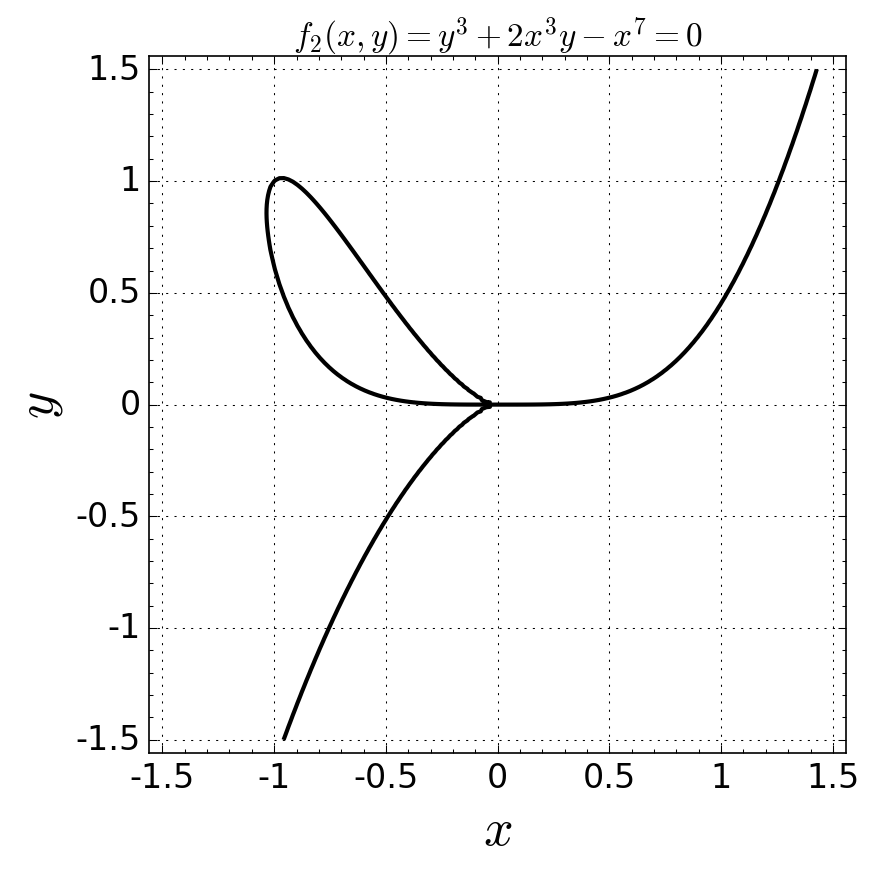
\includegraphics[width=0.5\textwidth]{images/f2.png}
  \caption{A real plot of the curve $C : f(x,y) = y^3 + 2 x^3 y - x^7$. The plot
    suggests that $(x_0 : x_1 : x_2) = (1 : 0 : 0)$, corresponding to $(x,y) =
    (0,0)$, is a singular point of $C$.}
  \label{fig: example-cubic}
\end{figure}

First, we find the finite singular points of $C$. Setting $a_0=1$ and solving
the above equations for $a_1$ and $a_2$ we see that $p = (1 : 0 : 0)$ is the
only finite singular point of $F$. Note that
\begin{gather*}
  f(x,y) = f_3(x,y) + f_4(x,y) + f_7(x,y), \\
  \\
  f_3(x,y) = y^3, \quad
  f_4(x,y) = 2 x^3 y, \quad
  f_7(x,y) = -x^7,
\end{gather*}
and that $f_3$, $f_4$, and $f_7$ are homogeneous of degrees 3, 4, and 7,
respectively. Therefore, $p$ is a singular point of multiplicity 3 with
\[
  f_3(x,y) = y^3 = 0,
\]
as the equation for the tangent cone at $p$. These properties are suggested by
Figure \ref{fig: example-cubic} where, near the point $p$, the real curve looks
like the intersection of three curves well approximated by the line $y = 0$ near
the point $x = 0$.

Setting $a_0 = 0$, the only expression in Equation \eqref{eq:
  singular-conditions} that does not reduce to zero is
\[
  \frac{\partial F}{\partial x_1}((0,a_1,a_2)) = - 7 a_{1}^{6} = 0,
\]
implying that the point $a = (0 : 0 : 1)$ is the only singular point at
infinity. The curve at infinity centered at $(0 : 0 : 1)$ is
\[
  h(w,z) = F(w,z,1) = w^{4} + 2 w^{3} z^{3} - z^{7}.
\]
The order of this singularity is four since this is the degree of the lowest
degree homogeneous term. The tangent cone at $a$ is $g_4(w,z) = w^4$.
\end{example}


%------------------------------------------------------------------------------
\subsection{Connection to Riemann Surfaces} \label{subsec:connection-to-riemann-surfaces}
%------------------------------------------------------------------------------

There is a close relationship between the study of compact Riemann surfaces and
that of algebraic curves. Recall that a Riemann surface $X$ is a complex
manifold of complex dimension one endowed with an {\it atlas}: an open covering
$\{U_\alpha \}_{\alpha \in A}$ of $X$ together with a collection of
homeomorphisms $\{z_\alpha : U_\alpha \to \CC\}_{\alpha \in A}$, called {\it
  local parameters}, such that every pair of {\it transition functions}
\[
  f_{\beta,\alpha} := z_\beta \circ z_\alpha^{-1} : z_\alpha \left( U_\alpha
    \cap U_\beta \right) \to z_\beta \left( U_\alpha \cap U_\beta \right),
\]
is holomorphic. The pairs $(U_\alpha, z_\alpha)$ are called {\it coordinate
  charts}. In other words, a Riemann surface is a topological space such that
for all $P \in X$ there is a neighborhood of $P$ homeomorphic to an open subset
of the complex plane and one can analytically continue from any $P \in X$ to any
$Q \in X$ via transition functions.

The Riemann sphere $X = \CC^*$ is an example of a Riemann surface. Its atlas
consists of two coordinate charts $(U_1, z_1)$ and $(U_2, z_2)$ with
\begin{align*}
  U_1 = \CC, & \quad z_1 = z, \\
  U_2 = \left( \CC - \{0\} \right) \cup \{ \infty \}, & \quad z_2 = 1/z.
\end{align*}
This is a valid atlas since the transition functions
\begin{gather*}
  f_{1,2}, f_{2,1} : \left(\CC - \{0\}\right)
  \to \left(\CC - \{0\}\right) \\
  f_{1,2} = z_1 \circ z_2^{-1} = 1/z \\
  f_{2,1} = z_2 \circ z_1^{-1} = 1/z
\end{gather*}
are holomorphic on $U_1 \cap U_2 = \CC - \{0\}$.

These relationships between curves and Riemann surfaces are embodied by the
following two theorems % TODO Griffiths reference

\begin{theorem} \label{thm: normalization} {\bf (Normalization Theorem.)} For
  any irreducible algebraic curve $C \subset \PP{2}\CC$ there exists a compact
  Riemann surface $X$ and a holomorphic mapping
  \[
    \sigma : X \to \PP{2}\CC,
  \]
  such that $\sigma( X ) = C$ and $\sigma$ is injective on the inverse image of
  the set of smooth points of $C$.
\end{theorem}

A Riemann surface together with the mapping $\sigma$ is called the {\it
  normalization of $C$}. Loosely speaking, the normalization theorem states that
an algebraic curve is a Riemann surface except at the singular points.

Conversely, every compact Riemann surface can be represented by an algebraic
curve.
\begin{theorem} \label{thm: repr-theorem} Any compact Riemann surface $X$ can be
  obtained through the normalization of a certain plane algebraic curve $C$ with
  at most ordinary double points. That is, there exists a holomorphic mapping
  \[
    \sigma : X \to \PP{2}\CC
  \]
  such that $\sigma(X)$ is an algebraic curve possessing at most ordinary double
  points.
\end{theorem}
Many of the geometric algorithms presented in this document are designed to
avoid singular points. Except, for example, when we want to integrate a 1-form
along a path leading to a singular point in which case we ``unwrap'' the
singularity using Puiseux series. This is discussed in more detail in the
following section. However, because of this we use the terms ``curve'' and
``Riemann surface'' interchangably.

Additionally, the algorithms presented in this document primarily work with the
affine part $f(x,y)$ of the curve $F(x_0,x_1,x_2)$. If analysis on the line at
infinity is necessary, for example, when computing the singular points of a
curve, we consider an affine projection $g$ of $F$ onto $l_\infty$,
\[
  g(u,y) = u^d f(1/u,y) = 0.
\]

Thus, the surface considered here is the branched algebraic $y$-covering of the
complex $x$-Riemann sphere, the set of all $(x,y)$-solutions to the affine
polynomial equation
\[
    C = \{ (x,y) \in \CC \; | \; f(x,y) = \alpha_d(x)y^d +
    \alpha_{d-1}y^{d-1} + \cdots + \alpha_1(x)y + \alpha_0(x) = 0\},
\]
as $x$ varies along all of $\CC$. We treat $x$ and $y$ as the independent and
dependent variables of the equation, respectively.

A {\it point} $\alpha \in \CC$ is called a {\it regular point of $C$} if
\[
  f(\alpha,y) = 0
\]
has $d$ distinct $y$-roots $y_0,\ldots,y_{d-1}$. A point $\alpha \in \CC$ is
called a discriminant point if it is not regular. The point $\alpha = \infty$ is
a regular point of $C$ if
\[
  g(0,y)
\]
has $d$ disctinct roots.

A {\it place} $P$ is an element of $X$. For all but finitely many places, $P$ is
given by a pair $(\alpha,\beta)$ such that $f(\alpha,\beta) = 0$. However, some
places, particularly those where $\alpha$ is a discriminant point, instead needs
to be represented by a pair of series $(x(t),y(t))$ in some local coordinate
$t$. This will be discussed in more detail in the following section.


%%%%%%%%%%%%%%%%%%%%%%%%%%%%%%%%%%%%%%%%%%%%%%%%%%%%%%%%%%%%%%%%%%%%%%%%%%%%%%%
\section{Algebraic Curves and Riemann
  Surfaces}\label{sec:background-algebraic-curves-and-riemann-surfaces}
%%%%%%%%%%%%%%%%%%%%%%%%%%%%%%%%%%%%%%%%%%%%%%%%%%%%%%%%%%%%%%%%%%%%%%%%%%%%%%%

In the previous section we introduced the Normalization Theorem relating complex
algebraic curves to Riemann surfaces. The goal of this section is to derive the
period matrix of a Riemann surface, the Abel Map, and the Riemann theta
function. These three objects are the primary ingredients in constructing a
large class of solutions to the Kadomtsev--Petviashvili equation, discussed in
\autoref{ch:kp}, and determinantal representations of plane curves, discussed in
\autoref{ch:determinantal}.

Throughout this section we present computational examples using the Sage
software package Abelfunctions \cite{abelfunctions}. Abelfunctions is a library
which provides general and easy to use framework for computing with Abelian
functions, Riemann surfaces, and algebraic curves. The reader may follow along
in the computations by downloading and installing Sage \cite{sage} from
\url{www.sagemath.org} and following the instructions on
\url{github.com/abefunctions/abelfunctions} for downloading and installing
Abelfunctions. See \autoref{ch:abelfunctions} for information on the algorithms
used and design of the software. In particular, an algorithmic perspective on
the below components can be found in \autoref{sec:abelfunctions-algorithms}.

\begin{figure}
\centering
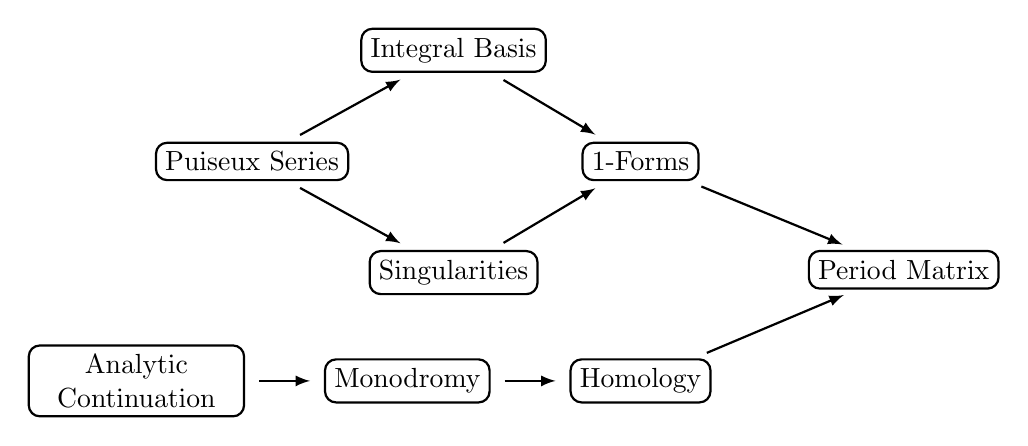
\begin{tikzpicture}
  \tikzstyle{element}=[rectangle, rounded corners, thick, draw]
  \tikzstyle{leadsto}=[->, shorten >=5pt, shorten <=5pt, >=latex, thick]

  % period matrix, abel map, and riemann constant vector
  \node[element] (periodmatrix) {Period Matrix};
  %\node[element] (abelmap) {Abel Map};
  %\node[element] (rcv) {Riemann Constant Vector};

  % dummy element to the left of period matrix
  \node[left=of periodmatrix, xshift=-1cm] (dummy) {};

  % = algebraic side =
  \node[element, above=of dummy] (oneforms) {1-Forms}
      edge [leadsto] (periodmatrix);
  \node[left=of oneforms, xshift=-0.5cm] (algdummy) {}; % alg dummy
  \node[element, above=of algdummy] (intbasis) {Integral Basis}
      edge [leadsto] (oneforms);
  \node[element, below=of algdummy] (singularities) {Singularities}
      edge [leadsto] (oneforms);
  \node[element, left=of algdummy,xshift=-0.2cm] (puiseux) {Puiseux Series}
      edge [leadsto] (singularities)
      edge [leadsto] (intbasis);

  % = geometric side =
  \node[element, below=of dummy] (homology) {Homology}
      edge [leadsto] (periodmatrix);
  \node[element, left=of homology] (monodromy) {Monodromy}
      edge [leadsto] (homology);
  \node[element, left=of monodromy, text width=2.5cm, align=center] (ancont) {Analytic Continuation}
      edge [leadsto] (monodromy);
\end{tikzpicture}
\caption{The major computations performed by {\tt abelfunctions} and
  their dependencies on one another.}
\label{fig: dependencies}
\end{figure}


The examples used in this chapter use the curves,
\begin{align}
  C_2 &:  f_2(x,y) = y^3 + 2x^3y - x^7 = 0, \label{eq:example-curve-f2} \\
  C_4 &:  f_4(x,y) = x^2y^3 - x^4 + 1 = 0. \label{eq:example-curve-f4}
\end{align}
In order to execute the code examples used in the rest of this chapter we begin
by starting Sage, importing Abelfunctions, and defining these two curves in
Sage,
\begin{lstlisting}
sage: from abelfunctions import *
sage: R.<x,y> = QQ['x,y']; R
Multivariate Polynomial Ring in x, y over Rational Field
sage: f2 = y^3 + 2*x^3*y - x^7
sage: X2 = RiemannSurface(f2)
sage: f4 = x^2*y^3 - x^4 + 1
sage: X4 = RiemannSurface(f4)
\end{lstlisting}


%%%%%%%%%%%%%%%%%%%%%%%%%%%%%%%%%%%%%%%%%%%%%%%%%%%%%%%%%%%%%%%%%%%%%%%%%%%%%%%
\subsection{Puiseux Series}\label{subsec:background-puiseux-series}
%%%%%%%%%%%%%%%%%%%%%%%%%%%%%%%%%%%%%%%%%%%%%%%%%%%%%%%%%%%%%%%%%%%%%%%%%%%%%%%

% ``From Riemann to Differential Geometry and Relativity''
\begin{quote}
  Victor Puiseux's modesty was intimidating, and his patience and politeness
  were admirable. To a student blundering at some test, he just used to say,
  with a very sweet tone: ``I don't know whether I heard well or whether I am
  mistaken, but it seems to me that what you said is not completely true.'' ---
  \'{E}mile Picard
\end{quote}

Every analytic function $f \in C^1(\RR)$ admits a local Taylor series
representation in a neighborhood about $x = \alpha$. If the function is
meromorphic it still admits a local series representation in the form of a
Laurent series,
\[
    f(x) = \sum_{n=N}^\infty c_n (x-\alpha)^n
\]
for some $N \in \ZZ \cup \{-\infty\}$ depending on $\alpha$. In both of these
situations the variable $x$ is a {\it local coordinate} of $f$ near the point
$\alpha$.

With algebraic curves, local coordinates are given in terms of Puiseux series
which can be thought of as an extension of Laurent series.
\begin{definition} \label{def: puiseux} A {\bf Puiseux series} expansion of a
  curve $C : f(x,y) = 0$ at the point $x=\alpha$ is a collection of $j =
  1,\ldots,m$ series, $m \leq d = \text{deg}_y f$, of the form
  \begin{align*}
    P_j(t) =
    \begin{cases}
      x_j(t) = \alpha + \lambda_j t^{e_j}, \\
      y_j(t) = \sum_{k=N}^\infty \beta_{jk} t^{n_{jk}},
    \end{cases}
  \end{align*}
  where $N \in \ZZ \cup \{-\infty\}$, $\alpha, \lambda_j, \beta_{jk} \in \CC$,
  and $e_j,n_{jk} \in \ZZ$. Each Puiseux series $P_j$ is called a {\bf place} on
  $C$. The variable, $t$, is called the {\bf local parameter} of the series and
  is centered at $t=0$.
\end{definition}
A place $P_j = P_j(t)$ satisfies,
\[
    f\big(P_j(t)\big) := f\big(x_j(t), y_j(t)\big) = 0.
\]
When a Puiseux series $P_j(t)$ represents an expansion about a non-singular
$(\alpha, \beta_j)$ on the curve then $P(0) = (\alpha,\beta)$. This is not
necessarily the case with singular places. We list some additional important
facts and properties of Puiseux series.
\begin{itemize}
\item The integer $|e_j|$ is called the {\it branching number} or {\it
    ramification index} of the series expansion at that place: $|e_j| > 1$ when
  $x = \alpha$ is a branch point of the curve. If $e_j = 1$ we say that the
  place is {\it unramified}.
\item The number of Puiseux series $m$ at a branch point $x = \alpha$ is less
  than or equal to $d = \text{deg}_y f$. In particular, $d = \sum_{j=1}^m
  |e_j|$. If $\alpha$ is not a branch point of the curve (see Section
  \ref{subsec:background-monodromy}) then $e_j = 1$ for all $j = 1, \ldots, d$;
  that is, there are $d$ unramified places above $x = \alpha$.
\item The field of Puiseux series is a splitting field for $\CC[x,y] =
  \CC[x][y]$. That is, given any $f \in \CC[x,y]$ and Puiseux series expansions
  about any $x=\alpha$ we can write
  \[
    f(x,y) = \prod_{j=1}^m \prod_{k=1}^{e_j} \left( y - y_j\left(
             (e/\lambda_j)^{2 \pi ik / e_j}(x-\alpha) \right) \right),
  \]
  where the first product ranges over all Puiseux series $P_j$ at $x=\alpha$ and
  the second product ranges over all $y$-components $y_j(x_j)$ when solving for
  $t$ in terms of $x$. Note that a Puiseux series $P_j$ with ramification index
  $|e_j|>1$ splits into $|e_j|$ $y$-series in $x$. Note that each unramified
  place has only one $x$-series representation; that is $P_j$ and $y_j$ are
  considered equivalent and in 1-1 correspondence.
\end{itemize}

\begin{example} \label{ex:f2-puiseux} Consider the example curve
  \[
    C_2 : f_2(x,y) = y^3 + 2x^3y - x^7 = 0.
  \]
  As seen in Example \ref{ex: 2-cubic}, the point $(x,y) = (0,0)$ is a singular
  point of $C$. The Puiseux series expansions lying above $x=0$ are,
  \begin{align} \label{eq:f2-puiseux-series-expansions}
    P_1(t) &= \begin{cases}
        x_1(t) = t, \\
        y_1(t) = \frac{t^{4}}{2} - \frac{t^{9}}{16} + \frac{3 t^{14}}{128} + O\left(t^{15}\right)
      \end{cases} \notag \\
    P_2(t) &= \begin{cases}
      x_2(t) = - \frac{t^{2}}{2}, \\
      y_2(t) =  - \frac{t^{3}}{2} - \frac{t^{8}}{64} + \frac{3 t^{13}}{4096} + O\left(t^{14}\right)
    \end{cases}
  \end{align}
  We see that $P_1$ is unramified and $P_2$ has ramification index of $2$. The
  sum of ramification indices of these two places is indeed $3 = \text{deg}_y
  f_2$. $P_2$ splits into two Puiseux $x$-series: solving for $x_2$ we get,
  \begin{equation}
    t = \pm \sqrt{2}i x^{1/2},
  \end{equation}
  which, when substituted into the expression for $y_2$ gives us,
  \begin{align}
    y_{2,+}(x) &= -\sqrt{2}ix^{3/2} - \tfrac{1}{4} x^4 - \tfrac{3\sqrt{2}}{64}x^{13/2} + O(x^{7}) \notag \\
    y_{2,-}(x) &= \sqrt{2}ix^{3/2} - \tfrac{1}{4} x^4 + \tfrac{3\sqrt{2}}{64}x^{13/2} + O(x^{7})
  \end{align}
  Substituting these truncated Puiseux series into affine expression of the
  curve we get,
  \begin{align}
    f_2\left(x_1(t), y_1(t)\right)
    &=
    \tfrac{3}{128}t^{22} - \tfrac{19}{4096}t^{27} + O\left(t^{32}\right) \notag \\
    f_2\left(x_2(t), y_2(t)\right)
    &=
      -\tfrac{3}{8192}t^{19} - \tfrac{1}{262144}t^{24} + O\left(t^{39}\right).
  \end{align}
  \begin{figure}
  \centering
  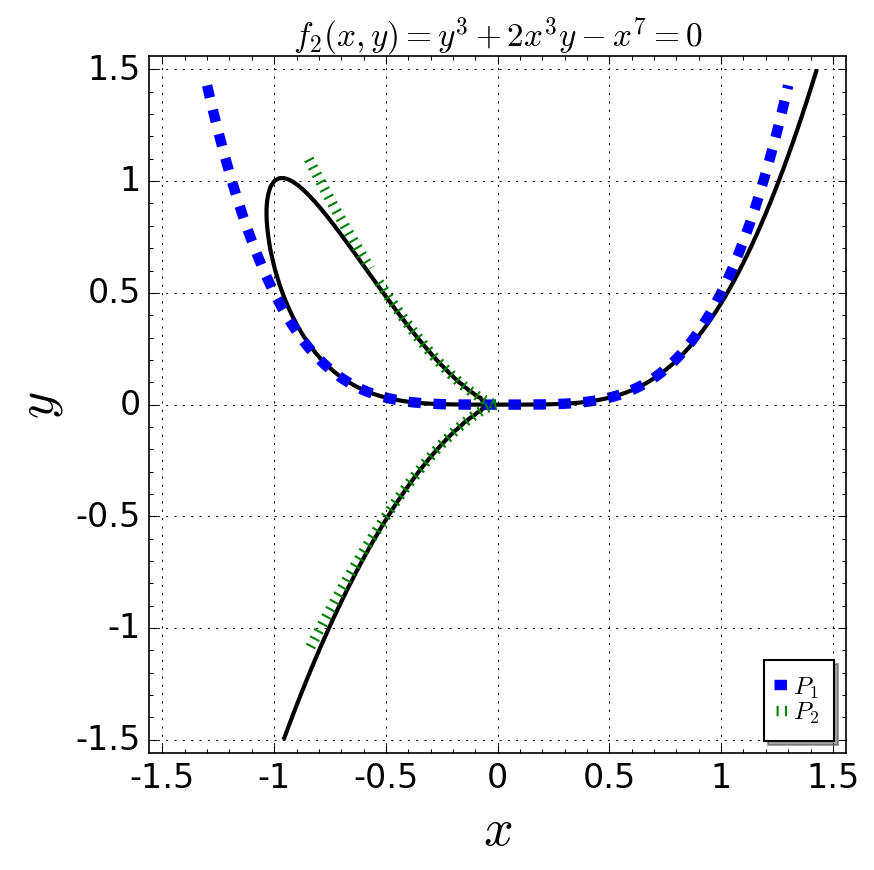
\includegraphics[width=0.49\textwidth]{images/f2-puiseux.png}
  \caption{A real plot of the curve $C_2: f_2(x,y) = y^3 + 2x^3y - x^7$. The
    blue and green dashed lines are plots of the places $P_1 = \left(t, t^4/2 +
      O(t^{9}) \right)$ and $P_2 = \left( -t^2/2, -t^3/2 + O(t^{8}) \right)$ for
    $t \in (-1.3, 1.3)$.}
  \label{fig:f2-puiseux}
  \end{figure}
  Again, the local parameter is always centered at $t=0$. Therefore, for small
  values of $|t|$ we see that $f_2\left(x(t), y(t)\right) = O(t^{19})$ is
  extraordinarily small in magnitude. As more terms are determined in the
  expansions of $y_1$ and $y_2$ we expect $N \to \infty$ in $f_2\left(x(t),
    y(t)\right) = O(t^N)$. We see that these series well-approximate the curve
  at $x=0$ in Figure \ref{fig:f2-puiseux}.
  
  We can verify these Puiseux series expansions above $x = 0$ and their
  properties using {\tt abelfunctions}.
  \begin{lstlisting}
  sage: P1, P2 = X2(0)  # the places above x=0 on the surface
  sage: P1
  (t, 1/2*t^4 + O(t^7))
  sage: P1.puiseux_series.extend(14)  # extend the curve to at least O(t^14)
  sage: P1
  (t, 1/2*t^4 - 1/16*t^9 + 3/128*t^14 + O(t^19))
  sage: P2
  (-1/2*t^2, -1/2*t^3 + O(t^5))
  sage: P2.puiseux_series.extend(13)  
  sage: P2  # may include higher order terms
  (-1/2*t^2, -1/2*t^3 - 1/64*t^8 + 3/4096*^13 - 1/16384*t^18 + O(t^20))
  \end{lstlisting}
\end{example}

\begin{example}
  Now consider the example curve,
  \[
    C_4 :  f_4(x,y) = x^2y^3 - x^4 + 1 = 0.
  \]
  \begin{figure}
  \centering
  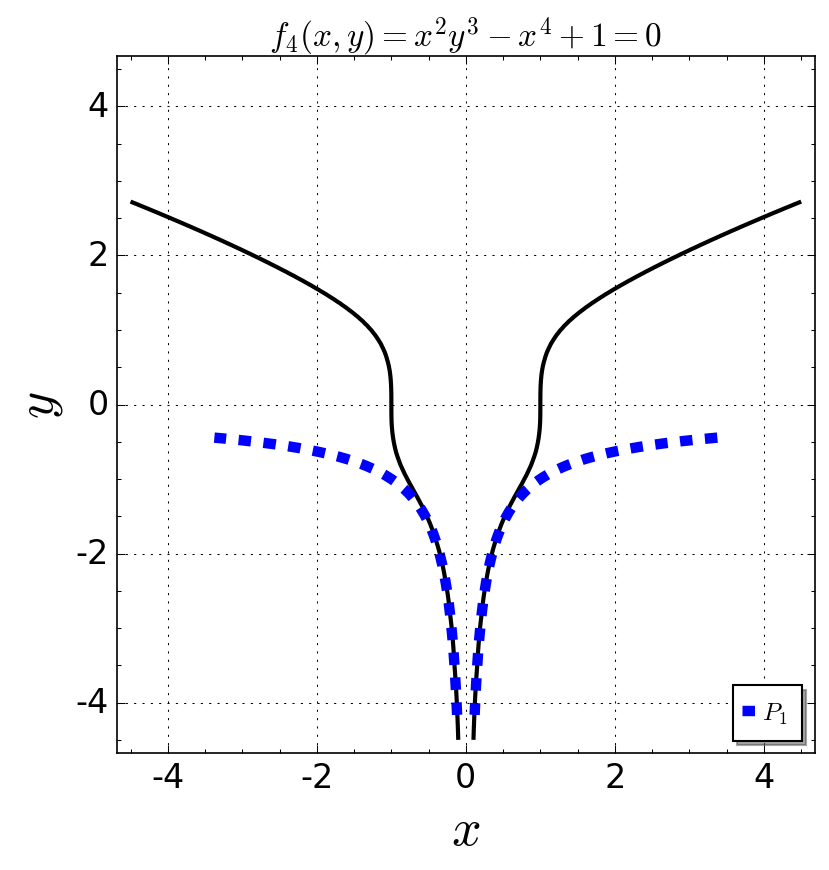
\includegraphics[width=0.49\textwidth]{images/f4-puiseux.png}
  \caption{A real plot of the curve $C_4: f_4(x,y) = x^2y^3 - x^4 + 1$. The
    dashed line is a plot of the place $P = \left(-t^3, -t^{-2} +
       O(t^{10})\right)$ for $t \in (-1.5, 1.5)$.}
  \label{fig:f4-puiseux}
  \end{figure}
  A plot of the curve in the real $x,y$-plane is shown in Figure
  \ref{fig:f4-puiseux}. There is a single place lying above $x=0$,
  \begin{equation}
    P(t) = \begin{cases}
      x(t) = -t^3, \\
      y(t) = -t^{-2} + \tfrac{1}{3}t^{10} + O(t^{15})
    \end{cases}
  \end{equation}
  Unlike the places shown in Example \ref{ex:f2-puiseux} the place $P$ has a
  component at infinity. The figure illustrates how $P$ acts as a local chart of
  the curve: the $O(t^{15})$ series expansion well-approximates the curve at
  $x=0$. In Abelfunctions, this place is treated like any other place.
  \begin{lstlisting}
  sage: P, = X4(0)
  sage: P  
  (-t^3, -t^-2 + O(t^0))
  sage: P.puiseux_series.extend(14)
  sage: P
  (-t^3, -t^-2 + 1/3*t^10 + O(t^15))
  \end{lstlisting}
\end{example}

Puiseux series expansions allow us to locally examine the behavior of an
algebraic curve or Riemann surface. In particular, they provide a local
coordinate chart centered at a point $(x,y) = (\alpha,\beta)$ on the curve in
the sense discussed in Section \ref{subsec:connection-to-riemann-surfaces}. In
the next section we describe a particular class of point/place on a Riemann
surface: the singular point.


%%%%%%%%%%%%%%%%%%%%%%%%%%%%%%%%%%%%%%%%%%%%%%%%%%%%%%%%%%%%%%%%%%%%%%%%%%%%%%%
\subsection{Singularities}\label{subsec:background-singularities}
%%%%%%%%%%%%%%%%%%%%%%%%%%%%%%%%%%%%%%%%%%%%%%%%%%%%%%%%%%%%%%%%%%%%%%%%%%%%%%%

Recall from Definition \ref{def: singular-point} that a point $a$ on a
projective curve $C$ is a singular point if
\[
  \left( \frac{\partial F}{\partial x_0}, \frac{\partial F}{\partial x_1},
    \frac{\partial F}{\partial x_2} \right) (a) = (0,0,0).
\]
For singular points of the form $a = (1 : \alpha, \beta)$, this is equivalent to
\[
  \frac{\partial f}{\partial x} (\alpha,\beta) = 0, \quad \frac{\partial
    f}{\partial y} (\alpha,\beta) = 0,
\]
where $f$ is the affine portion of the curve. The singular points of a curve
need to be determined not only for the numerical analytic continuation and
integration methods discussed below, so we can appropriately desingularize the
curve $C$ and obtain a Riemann surface $X$, but they are also an essential
ingredient to computing a basis of holomorphic 1-forms on $X$.

For singular points of the form $a = (1 : \alpha : \beta)$ the Puiseux series
expansion $P_j$ of $f = f(x,y)$ such that $P_j(0) = (\alpha, \beta)$ is a
coordinate chart centered at $(x,y) = (\alpha, \beta)$. $P_j$ tells us how to
approach and pass through $(x,y) = (\alpha, \beta)$ on the curve. Similarly,
singular points at infinity have coordinate charts defined by the Puiseux series
with $e_j < 0$. With these coordinate charts we can desingularize the curve and
thus create an appropriate atlas for the corresponding Riemann surface $X$.

For the purposes of later determining the genus of $X$ as well as the space of
holomorphic 1-forms $\Gamma(X,\Omega_X^1)$ on $X$ we need to compute the {\it
  delta invariant} and the {\it multiplicity} of a singularity. In the following
discussion we assume for simplicity that the singularity is finite. To analyze
infinite singular points we project the curve $C$ onto the line at infinity
$l_\infty$ using the method described in Section \ref{sec:
  projective-plane-curves}.

\begin{itemize}
\item {\bf branching number} --- The branching number $R$ of a singular point
  $(\alpha, \beta)$ is the sum of the branching numbers/ramification indices of
  the Puiseux series centered at $(x,y) = (\alpha,\beta)$. That is,
  \begin{equation} \label{eq:branching-number}
    R = \!\!\!\! \sum_{\substack{j \\ P_j(0)=(\alpha,\beta)}} |e_j|.
  \end{equation}
\item {\bf multiplicity} --- As given in Section \ref{sec:
    projective-plane-curves}, the multiplicity of a singular point is the degree
  of the lowest degree non-zero homogeneous term appearing in the polynomial
  expression for the curve centered at $(\alpha, \beta)$.
\item {\bf delta invariant} --- The delta invariant $\delta_P$ of a singularity
  $P$ is the number of double points concentrated at the singularity. This is
  equal to the number of quadratic factors $(\alpha_i x - \beta_i y)^2$
  appearing in the tangent cone at the singularity. Let $S$ be the set of all
  singular points, finite and infinity, of $C$. Then the genus is given by
  \begin{equation} \label{eq:genus-formula}
    g = \frac{(d-1)(d-2)}{2} - \sum_{P \in S} \delta_P.
  \end{equation}
\end{itemize}

\begin{example}
  We compute the singularities of the curve,
\[
  C_2 : f_2(x,y) = y^3 + 2x^3y - x^7 = 0.
\]
Note that to match the notation used in Sage the finite and infinite
singularities are presented in the format $(\alpha : \beta : 1)$ and $(\gamma :
1 : 0)$, respectively. The order of the projective components is different than
that presented in Section \ref{sec:projective-plane}.
\begin{lstlisting}
sage: S = singularities.singularities(f2)
sage: for s, (m, delta, r) in S:
....:     print 'Singularity:', s
....:     print '\tmultiplicity     =', m
....:     print '\tdelta invariant  =', delta
....:     print '\tbranching number =', r
....:
Singularity: (0, 0, 1)
	multiplicity     = 3
	delta invariant  = 4
	branching number = 2
Singularity: (0, 1, 0)
	multiplicity     = 4
	delta invariant  = 9
	branching number = 1
\end{lstlisting}
As seen in Equation \eqref{eq:f2-puiseux-series-expansions} the places $P_1$ and
$P_2$ above $x=0$, which have $y-$component $y(0) = 0$, have ramification
indices 1 and 2, respectively, which matches the expected multiplicity. HOLY
SHIT! THERE MAY BE AN ISSUE, HERE.

The genus is computed using the formula in Equation \eqref{eq:genus-formula}.
Later, performs additional checks on the genus using the geometric properties
discussed in \ref{subsec:background-monodromy}.
\begin{lstlisting}
sage: singularities.genus(f,x,y)
2  
\end{lstlisting}
\end{example}

\begin{example}
We compute the singularities of the curve,
\[
  C : f(x,y) = (y^2-x^2)(x-1)(2x-3) - 4(x^2+y^2-2x)^2.
\]
\begin{figure}
  \centering
  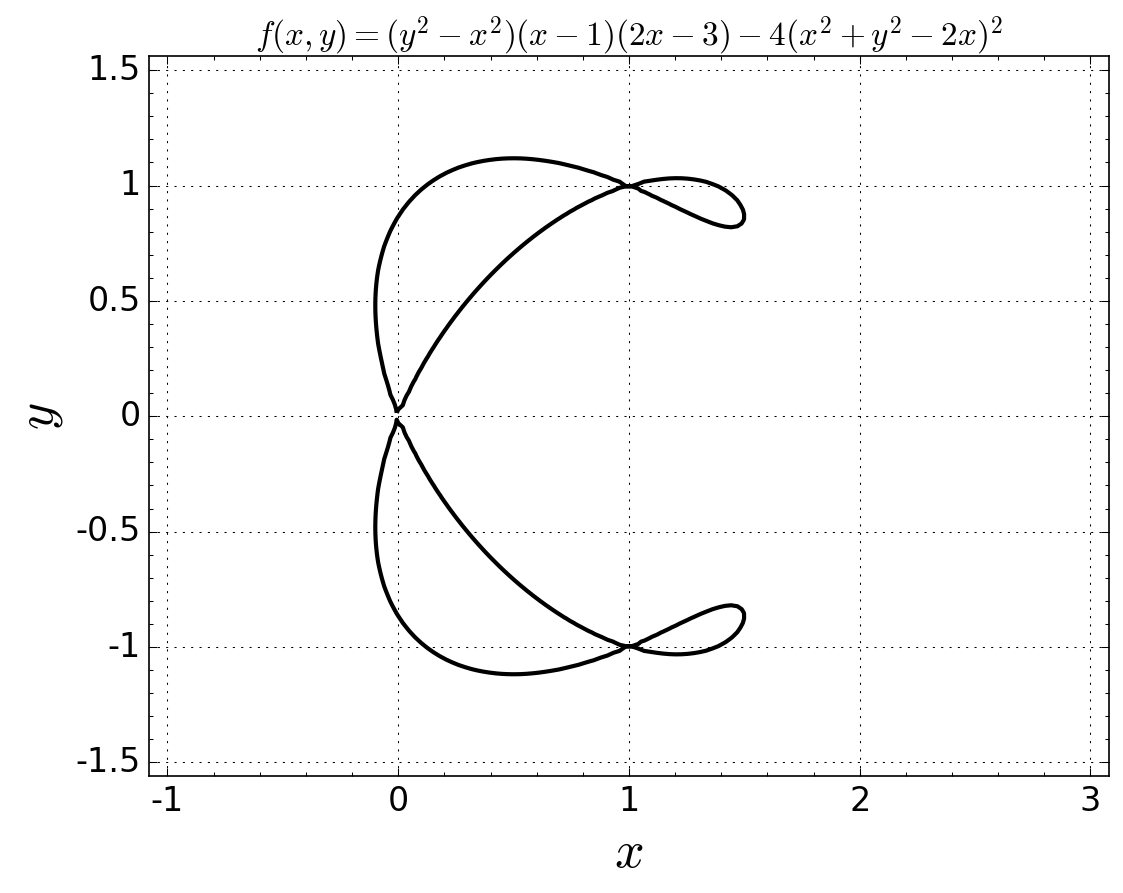
\includegraphics[width=0.49\textwidth]{images/f-singularities-example.png}
  \caption{A real plot of the curve $C: f(x,y) = (y^2-x^2)(x-1)(2x-3) -
    4(x^2+y^2-2x)^2$. Note the singularities at $(0,0), (1,1),$ and $(1,-1)$
    where the gradient vanishes.}
  \label{fig:f-singularities-example}
\end{figure}
A plot of the curve in the real $x,y$-plane is shown in Figure
\ref{fig:f-singularities-example}. The gradient of the curve in the affine plane
is given by,
\[
  \nabla f(x,y) = \left(
    -(12x-11)y^2 -24x^3 + 63x^2 - 38x, \quad
    -16y^3 - 2(6x^2 - 11x - 3)y
  \right).
\]
The gradient indeed vanishes at the points $(x,y) = (0,0), (1,1),$ and $(1,-1)$.
In fact, these are the only singular points of this curve.
\begin{lstlisting}
sage: f = (y^2-x^2)*(x-1)*(2*x-3) - 4*(x^2+y^2-2*x)^2
sage: S = singularities.singularities(f4)
sage: for s, (m, delta, r) in S:
....:     print 'Singularity:', s
....:     print '\tmultiplicity     =', m
....:     print '\tdelta invariant  =', delta
....:     print '\tbranching number =', r
....:
Singularity: (0, 0, 1)
	multiplicity     = 2
	delta invariant  = 1
	branching number = 2
Singularity: (1, -1, 1)
	multiplicity     = 2
	delta invariant  = 1
	branching number = 2
Singularity: (1, 1, 1)
	multiplicity     = 2
	delta invariant  = 1
	branching number = 2
\end{lstlisting}
This curve is a rational curve: the total degree of the curve is $d=4$ and the
three singularities have a delta invariant equal to one.
\end{example}


%%%%%%%%%%%%%%%%%%%%%%%%%%%%%%%%%%%%%%%%%%%%%%%%%%%%%%%%%%%%%%%%%%%%%%%%%%%%%%%
\subsection{Analytic Continuation}\label{subsec:background-analytic-continuation}
%%%%%%%%%%%%%%%%%%%%%%%%%%%%%%%%%%%%%%%%%%%%%%%%%%%%%%%%%%%%%%%%%%%%%%%%%%%%%%%

\begin{quote}
  The description of right lines and circles, upon which geometry is founded,
  belongs to mechanics. Geometry does not teach us to draw these lines, but
  requires them to be drawn. --- Isaac Newton
\end{quote}

The root of our geometric approach toward the period matrix of a Riemann surface
are paths on the Riemann surface. A {\it path on a Riemann surface, $X$,} is a
continuous map $\gamma : [0,1] \to X$. On the normalization of a curve $C:
f(x,y) = 0$ a path can be defined as $\gamma : [0,1] \to C \subset \CC^2$. That
is, if $\gamma(t) = (x_\gamma(t), y_\gamma(t))$ then $f(x(t),y(t)) = 0$ for all
$t \in [0,1]$. The roots of a polynomial are continuous as a function of the
coefficients. Therefore, an $x$-path $x_\gamma : [0,1] \to \CC_x$ and an initial
$y$-root $y_0 \in \CC_y$ are sufficient for defining a path on $C$ for the
resulting $y$-path $y_\gamma : [0,1] \to \CC_y$ is completely determined by the
curve
\[
  f(x_\gamma(t),y) = 0.
\]
The process of deriving this $y$-path from the data provided is referred to as
{\it analytic continuation}.

A {\it closed path $\gamma$ on a Riemann surface} is one such that $\gamma(0) =
\gamma(1)$. That is, a path is closed when $x_\gamma(0) = x_\gamma(1)$ and
$y_\gamma(0) = y_\gamma(1)$. When constructing a path using an $x$-path it may
be the case that the $x$-path $x_\gamma(t)$ is closed in $\CC_x$ but the derived
$y$-path $y_\gamma(t)$ may not satisfy $y_\gamma(0) = y_\gamma(1)$. This
situation is described in more detail in Section \ref{sec: monodromy} on
monodromy groups of algebraic curves.


%%%%%%%%%%%%%%%%%%%%%%%%%%%%%%%%%%%%%%%%%%%%%%%%%%%%%%%%%%%%%%%%%%%%%%%%%%%%%%%
\subsection{Monodromy}\label{subsec:background-monodromy}
%%%%%%%%%%%%%%%%%%%%%%%%%%%%%%%%%%%%%%%%%%%%%%%%%%%%%%%%%%%%%%%%%%%%%%%%%%%%%%%

At a generic point $x = \alpha_0 \in \CC$ a curve $C : f(x,y) = 0$ has $d$
distinct ordered $y$-roots $(y_0,\ldots,y_{d-1})$ at $\alpha_0$. This collection
of $y$-roots is sometimes called the {\it lift of} or the {\it fibre above}
$x=\alpha_0$. However, at a point $x=b$ where both $f(x,y) = 0$ and $\partial_y
f(x,y) = 0$ the number of distinct roots in the lift is strictly less than $d$.
Such a point $x = b$ is called a {\it discriminant point} of $f$.

A {\it branch point} $x=b$ is a discriminant point having the property that if
one were to analytically continue an ordered fibre around some closed path
encircling $b$ then the elements of the fibre are permuted. Specifically, let
$x_{\gamma} : [0,1] \to \CC$ be a piecewise differentiable oriented closed path
in the complex $x$-plane encircling a branch point $x=b$ exactly once in the
positive direction and let $(y_0,\ldots,y_{d-1})$ be a fixed ordering of the
fibre at $x_\gamma(0) = b$. Then, after analytically continuing the fibre around
$x_\gamma$ and returning to $x_\gamma(1) = b$, the fibre is equal to
\[
    (y_{\pi_b(0)}, \ldots, y_{\pi_b(d-1)}),
\]
where $\pi_b \in S_d$ is a permutation on $d$ elements. In other wods, a
{\it branch point} is a discriminant point with $\pi_b \neq \text{id}$.

To analyze the permutation behavior of multiple branch points
$\{b_1,\ldots,b_n\}$ we start by fixing some {\it base point} $x=\alpha_0$ in
the complex plane such that $\alpha_0$ is not a branch point and we fix an
ordering $(y_0,\ldots,y_{d-1})$ of the fibre above $\alpha_0$. Let $x_{\gamma_k}
: [0,1] \to \CC$ be a path encircling only the branch point $b_k$ in the
positive direction which does not cross the other paths. Such a path is called a
{\it monodromy path} of $b_k$. In the case when $x = \infty$ is a branch point a
monodromy path for $\infty$ is taken to be a circle going around all of the
finite branch points in the negative direction. See Figure \ref{fig: mon} for an
illustration of these paths.

\begin{figure}
  \centering
%  \includegraphics[width=0.6\textwidth]{images/mon.png}

  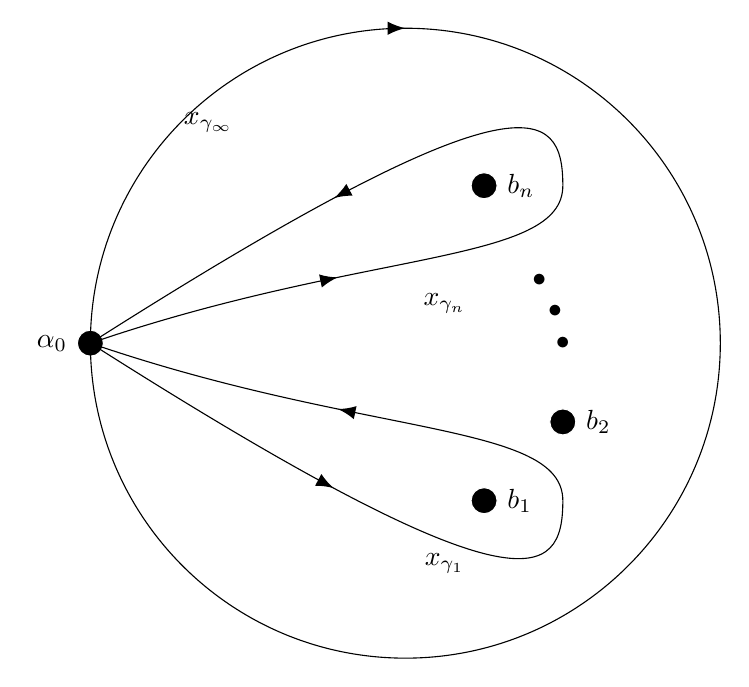
\begin{tikzpicture}
    \tikzstyle{discpt}=[circle,draw=white,fill=black,thin,minimum size=2pt,
                        radius=2pt]
    \tikzstyle{monpath}=[decoration={markings,
        mark=at position 0.5 with {\arrow[very thick]{latex}}},
      postaction={decorate}]

    % draw the discriminant points and interpolating dots
    \node[discpt] (b1) at (-1,-2)     [label=right:$b_1$] {};
    \node[discpt] (b2) at (0,-1)      [label=right:$b_2$] {};
    \node at (0,0) {$\bullet$};
    \node at (-0.1,0.4) {$\bullet$};
    \node at (-0.3,0.8) {$\bullet$};
    \node[discpt] (bn) at (-1,2)     [label=right:$b_n$] {};
    \node[discpt] (a) at (-6,0)      [label=left:$\alpha_0$] {};

    % the oriented paths
    \draw[monpath] (-6,0) ..
                   controls (-0.5,-3.5) and (0,-3) ..
                   (0,-2);
    \draw[monpath] (0,-2) ..
                   controls (0,-1) and (-2.5,-1.2) ..
                   (-6,0);
    \node at (-1.5,-2.8) {$x_{\gamma_1}$};

    \draw[monpath] (-6,0) ..
                   controls (-2.5,1.2) and (0,1) ..
                   (0,2);
    \draw[monpath] (0,2) ..
                   controls (0,3) and (-0.5,3.5) ..
                   (-6,0);
    \node at (-1.5,0.5) {$x_{\gamma_n}$};

    % path around infinity
    \draw[monpath] (-6,0) arc (180:0:4);
    \draw          (2,0) arc (0:-180:4);
    \node at (-4.5,2.8) {$x_{\gamma_\infty}$};

    %% \begin{scope}[very thick]
    %% \end{scope}
  \end{tikzpicture}
  \caption{The discriminant points $b_1,\ldots,b_n$ with their
    respective monodromy paths $x_{\gamma_1}, \ldots, x_{\gamma_n}$ and
    the path $x_{\gamma_\infty}$ around the point at infinity.}
  \label{fig: mon}
\end{figure}

Analytically continuing the ordered fibre $(y_0, \ldots, y_{d-1})$ around each
of the branch points results in $n+1$ permutations
\[
  \pi_{b_1}, \ldots, \pi_{b_n}, \pi_\infty \in S_d
\]
The group generated by these permutations is called the {\it fundamental group}
of $\CC \backslash \{b_1, \ldots, b_n\}$. It is denoted $\pi_1(\PP{1}\CC
\backslash \{b_1, \ldots, b_n\}, \alpha_0).$ Observe that, by the disjoint path
condition on the monodromy paths, moving the base point $\alpha_0$ corresponds
to conjugation of the generators of the fundamental group by some $\pi \in S_d$.
Hence, the monodromy group has explicit dependence on the base point.


We compute the monodromy group of the curve
\[
  C : f(x,y) = y^3 + 2x^3y - x^7 = 0,
\]
where the permutations $\pi_j \in \pi_1(\PP{1}\CC \backslash \{b_1, \ldots,
b_n\}, \alpha_0)$ are presented in disjoint cycle notation.
\begin{lstlisting}
from abelfunctions import *
from sympy.abc import x,y,t

f = y**3 + 2*x**3*y - x**7
X = RiemannSurface(f,x,y)

b = X.branch_points()
pi_1 = X.monodromy_group()

for bj,pi_1j in zip(b,pi_1):
    print 'branch point:', bj
    print 'permutation: ', pi_1j
    print
\end{lstlisting}
\begin{lstlisting}
branch point: (-0.31969776999-0.983928563571j)
permutation:  [(0, 2), (1,)]

branch point: (0.836979627962-0.608101294789j)
permutation:  [(0,), (1, 2)]

branch point: (-1.03456371594+0j)
permutation:  [(0,), (1, 2)]

branch point: 0j
permutation:  [(0, 2), (1,)]

branch point: (0.836979627962+0.608101294789j)
permutation:  [(0,), (1, 2)]

branch point: (-0.31969776999+0.983928563571j)
permutation:  [(0, 1), (2,)]

branch point: oo
permutation:  [(0, 2, 1)]
\end{lstlisting}
The method \verb=RiemannSurface.show_paths()= plots all the monodromy paths
$x_{\gamma_j}$ in the complex $x$-plane. The base point $x=\alpha_0$ is marked
in red.
\begin{lstlisting}[firstnumber=14]
X.show_paths()
\end{lstlisting}
\begin{lstlisting}
<matplotlib.figure.Figure object at 0x107d60810>
\end{lstlisting}
\begin{center}
%TODO \includegraphics[width=0.75\textwidth]{images/monexample.pdf}
\end{center}


%%%%%%%%%%%%%%%%%%%%%%%%%%%%%%%%%%%%%%%%%%%%%%%%%%%%%%%%%%%%%%%%%%%%%%%%%%%%%%%
\subsection{Homology}\label{subsec:background-homology}
%%%%%%%%%%%%%%%%%%%%%%%%%%%%%%%%%%%%%%%%%%%%%%%%%%%%%%%%%%%%%%%%%%%%%%%%%%%%%%%

A compact Riemann surface $X$ of genus $g$ is homeomorphic to a sphere with $g$
handles or, equivalently, a doughnut with $g$ holes. A cycle on $X$ is a closed,
oriented, piecewise smooth curve $\gamma : [0,1] \to X$ such that $\gamma(0) =
\gamma(1)$. The first homology group $H_1(X,\ZZ)$ of $X$ is the collection of
all cycles on $X$ modulo homologous transformations. In this document we do not
state precisely what it means for two cycles to be homologous since it involves
presenting the basic theory of simplicial complexes which is beyond the scope of
this document.

However, in brief, two cycles on $X$ are homologous if they can be deformed to
each other where the process of deformation not only allows continuous
transformations but the splitting of one cycle into two via ``pinching''. A
demonstration of this procedure is shown in Figure \ref{fig: pinching}. Two
cycles can be added together by ``reversing'' the pinching process and negation
of a path corresponds to reversing its orientation. The {\it first homology
  group} $H_1(X,\ZZ)$ is the set of all cycles on $X$ with the addition
operation described. The equivalence of cycles on a Riemann surface is the same
as that of closed paths on the complex plane (specifically, the Riemann sphere)
upon which one integrate a fixed meromorphic function $g$. Closed paths not
encircling a pole of $g$ are homologous to the zero path since they can be
contracted to a point. The set of all paths encircling a single, given pole are
all homologous to each other.

\begin{figure}
  \centering
  %
  % ONE BIG PATH
  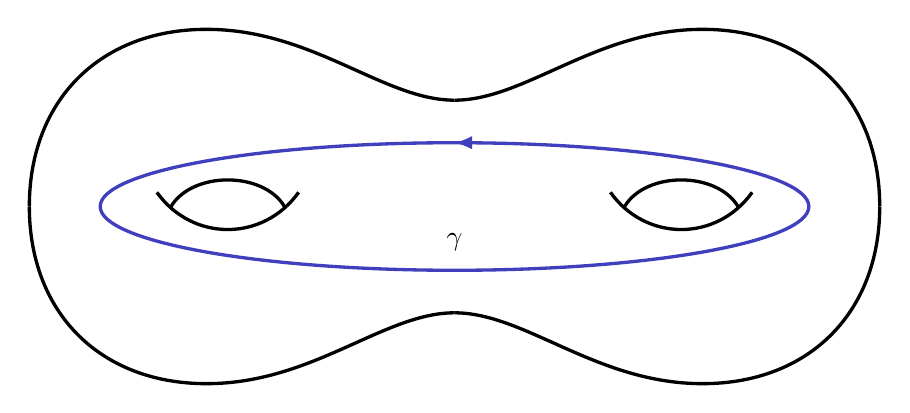
\begin{tikzpicture}[scale=0.9]
    \colorlet{darkgreen}{green!50!gray}
    \colorlet{darkblue}{blue!50!gray}

    \begin{scope}[very thick]
    % Quadrant II of Torus
    % (other draw statements are flips / rotations)
    \draw (-6,0) ..
          controls (-6,1.5) and (-5,2.5) ..
          (-3.5,2.5) ..
          controls (-2,2.5) and (-1,1.5) ..
          (0,1.5);
    \draw[xscale=-1] (-6,0) ..
          controls (-6,1.5) and (-5,2.5) ..
          (-3.5,2.5) ..
          controls (-2,2.5) and (-1,1.5) ..
          (0,1.5);
    \draw[rotate=180] (-6,0) ..
          controls (-6,1.5) and (-5,2.5) ..
          (-3.5,2.5) ..
          controls (-2,2.5) and (-1,1.5) ..
          (0,1.5);
    \draw[yscale=-1] (-6,0) ..
          controls (-6,1.5) and (-5,2.5) ..
          (-3.5,2.5) ..
          controls (-2,2.5) and (-1,1.5) ..
          (0,1.5);

    % The Holes
    % (one hole at center shifted to outsides)
    \draw[xshift=-3.2cm] (-0.8,0) ..
          controls (-0.5,0.5) and (0.5,0.5) ..
          (0.8,0);
    \draw[yscale=-1,xshift=-3.2cm] (-1,-0.2) ..
          controls (-0.5,0.5) and (0.5,0.5) ..
          (1,-0.2);

    \draw[xshift=3.2cm] (-0.8,0) ..
          controls (-0.5,0.5) and (0.5,0.5) ..
          (0.8,0);
    \draw[yscale=-1,xshift=3.2cm] (-1,-0.2) ..
          controls (-0.5,0.5) and (0.5,0.5) ..
          (1,-0.2);

    % sum of paths example
    % gamma
    \draw[darkblue, decoration={markings,
              mark=at position 0.25 with {\arrow[very thick]{latex}}},
          postaction={decorate}]
    (0,0) ellipse (5cm and 0.9cm);
    \draw (0,-0.5) node {$\gamma$};
    \end{scope}
  \end{tikzpicture}

  \vspace{24pt}

  %
  % PINCHING THE PATHS
  %
  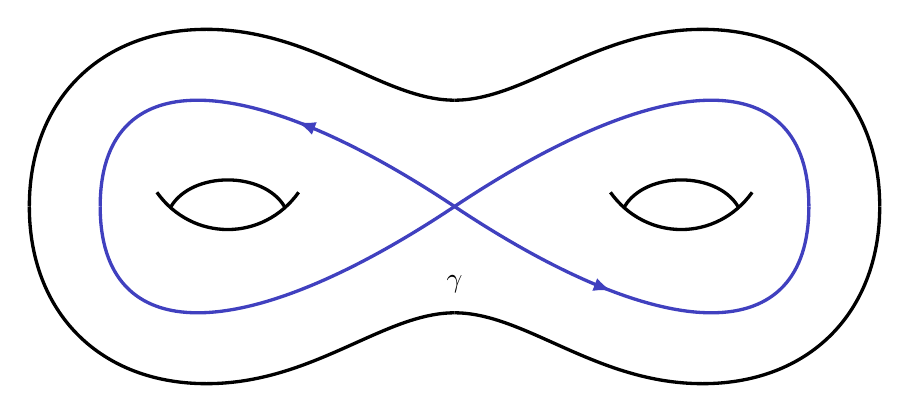
\begin{tikzpicture}[scale=0.9]
    \colorlet{darkgreen}{green!50!gray}
    \colorlet{darkblue}{blue!50!gray}

    \begin{scope}[very thick]
    % Quadrant II of Torus
    % (other draw statements are flips / rotations)
    \draw (-6,0) ..
          controls (-6,1.5) and (-5,2.5) ..
          (-3.5,2.5) ..
          controls (-2,2.5) and (-1,1.5) ..
          (0,1.5);
    \draw[xscale=-1] (-6,0) ..
          controls (-6,1.5) and (-5,2.5) ..
          (-3.5,2.5) ..
          controls (-2,2.5) and (-1,1.5) ..
          (0,1.5);
    \draw[rotate=180] (-6,0) ..
          controls (-6,1.5) and (-5,2.5) ..
          (-3.5,2.5) ..
          controls (-2,2.5) and (-1,1.5) ..
          (0,1.5);
    \draw[yscale=-1] (-6,0) ..
          controls (-6,1.5) and (-5,2.5) ..
          (-3.5,2.5) ..
          controls (-2,2.5) and (-1,1.5) ..
          (0,1.5);

    % The Holes
    % (one hole at center shifted to outsides)
    \draw[xshift=-3.2cm] (-0.8,0) ..
          controls (-0.5,0.5) and (0.5,0.5) ..
          (0.8,0);
    \draw[yscale=-1,xshift=-3.2cm] (-1,-0.2) ..
          controls (-0.5,0.5) and (0.5,0.5) ..
          (1,-0.2);

    \draw[xshift=3.2cm] (-0.8,0) ..
          controls (-0.5,0.5) and (0.5,0.5) ..
          (0.8,0);
    \draw[yscale=-1,xshift=3.2cm] (-1,-0.2) ..
          controls (-0.5,0.5) and (0.5,0.5) ..
          (1,-0.2);

    % sum of paths example
    % gamma_1
    \draw[darkblue, decoration={markings,
          mark=at position 0.4 with {\arrow[very thick]{latex}}},
          postaction={decorate}]
          (0,0) ..
          controls (3,-2) and (5,-2) ..
          (5,0);
    \draw[darkblue]
          (5,0) ..
          controls (5,2) and (3,2) ..
          (0,0);

    \draw[darkblue, decoration={markings,
          mark=at position 0.4 with {\arrow[very thick]{latex}}},
          postaction={decorate}]
          (0,0) ..
          controls (-3,2) and (-5,2) ..
          (-5,0);
    \draw[darkblue]
          (-5,0) ..
          controls (-5,-2) and (-3,-2) ..
          (0,0);
    \draw (0,-1.1) node {$\gamma$};
    \end{scope}
  \end{tikzpicture}

  \vspace{24pt}

  %
  % SEPARATING THE PATHS
  %
  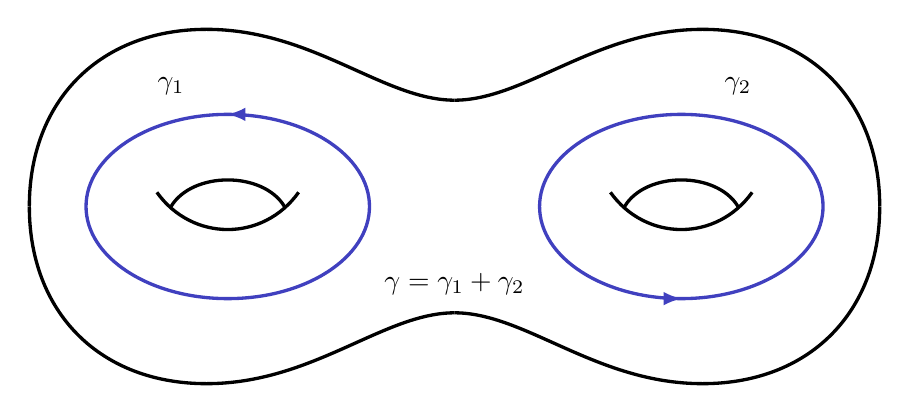
\begin{tikzpicture}[scale=0.9]
    \colorlet{darkgreen}{green!50!gray}
    \colorlet{darkblue}{blue!50!gray}

    \begin{scope}[very thick]
    % Quadrant II of Torus
    % (other draw statements are flips / rotations)
    \draw (-6,0) ..
          controls (-6,1.5) and (-5,2.5) ..
          (-3.5,2.5) ..
          controls (-2,2.5) and (-1,1.5) ..
          (0,1.5);
    \draw[xscale=-1] (-6,0) ..
          controls (-6,1.5) and (-5,2.5) ..
          (-3.5,2.5) ..
          controls (-2,2.5) and (-1,1.5) ..
          (0,1.5);
    \draw[rotate=180] (-6,0) ..
          controls (-6,1.5) and (-5,2.5) ..
          (-3.5,2.5) ..
          controls (-2,2.5) and (-1,1.5) ..
          (0,1.5);
    \draw[yscale=-1] (-6,0) ..
          controls (-6,1.5) and (-5,2.5) ..
          (-3.5,2.5) ..
          controls (-2,2.5) and (-1,1.5) ..
          (0,1.5);

    % The Holes
    % (one hole at center shifted to outsides)
    \draw[xshift=-3.2cm] (-0.8,0) ..
          controls (-0.5,0.5) and (0.5,0.5) ..
          (0.8,0);
    \draw[yscale=-1,xshift=-3.2cm] (-1,-0.2) ..
          controls (-0.5,0.5) and (0.5,0.5) ..
          (1,-0.2);

    \draw[xshift=3.2cm] (-0.8,0) ..
          controls (-0.5,0.5) and (0.5,0.5) ..
          (0.8,0);
    \draw[yscale=-1,xshift=3.2cm] (-1,-0.2) ..
          controls (-0.5,0.5) and (0.5,0.5) ..
          (1,-0.2);

    % sum of paths example
    \draw[xshift=-3.2cm, darkblue, decoration={markings,
              mark=at position 0.25 with {\arrow[very thick]{latex}}},
          postaction={decorate}]
         (0,0) ellipse (2cm and 1.3cm);
    \draw[xshift=3.2cm, darkblue, decoration={markings,
              mark=at position 0.75 with {\arrow[very thick]{latex}}},
          postaction={decorate}]
         (0,0) ellipse (2cm and 1.3cm);

    \draw (0,-1.1) node {$\gamma = \gamma_1 + \gamma_2$};\
    \draw (-4,1.7)  node {$\gamma_1$};
    \draw (4,1.7)   node {$\gamma_2$};
    \end{scope}
  \end{tikzpicture}
  \caption{A genus $g=2$ Riemann surface $X$ with three homologous cycles. The
    process of ``pinching'' and separating a cycle $\gamma$ into two cycle is
    allowed. Cycles can be added together by reversing this pinching process.
    Negation of a cycle corresponds to reversing its orientation.}
  \label{fig: pinching}
\end{figure}

$H_1(X,\ZZ)$ has a basis of cycles $\{a_1,\ldots,a_g,b_1,\ldots,b_g\}$. That is,
every cycle on $X$ can be written as a finite, integer linear combination of the
$a$- and $b$-cycles. These cycles can be chosen such that they satisfy the
intersection properties
\begin{gather*}
  a_i \circ a_j = 0, \quad \forall i \neq j \\
  b_i \circ b_j = 0, \quad \forall i \neq j \\
  a_i \circ b_j = \delta_{ij}, \quad \forall i,j = 1, \ldots, g
\end{gather*}
where $\delta_{ij}$ is the Kronecker delta. That is, the only cycles that
intersect are $a_i$ and $b_i$. A basis of cycles fulfilling these intersection
requirements is called a {\it canonical basis of cycles}. Figure \ref{fig:
  cycle-basis} illustrates the canonical basis for a genus two Riemann surface.

\begin{figure}
  \centering
  %
  % DEMONSTRATION OF BASIS CYCLES
  %
  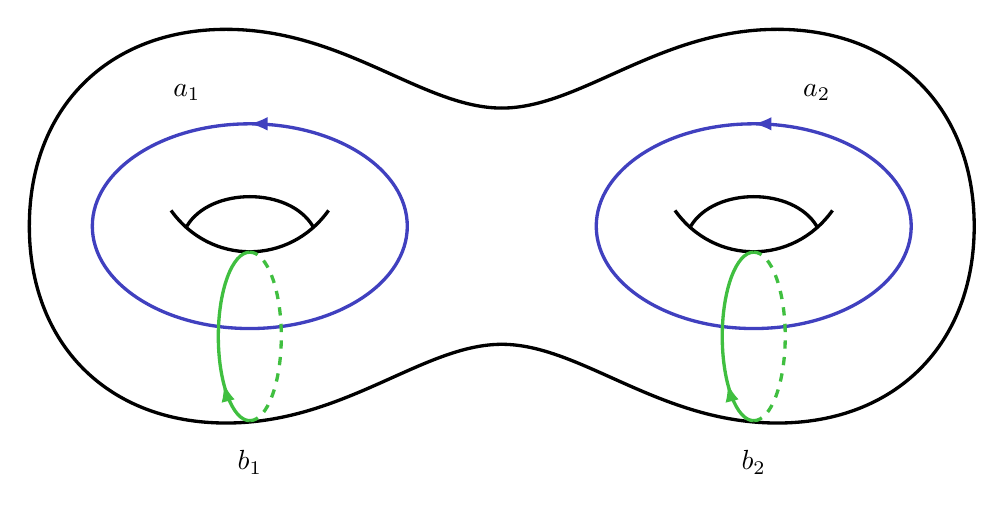
\begin{tikzpicture}
    \colorlet{darkgreen}{green!50!gray}
    \colorlet{darkblue}{blue!50!gray}

    \begin{scope}[very thick]
    % Quadrant II of Torus
    % (other draw statements are flips / rotations)
    \draw (-6,0) ..
          controls (-6,1.5) and (-5,2.5) ..
          (-3.5,2.5) ..
          controls (-2,2.5) and (-1,1.5) ..
          (0,1.5);
    \draw[xscale=-1] (-6,0) ..
          controls (-6,1.5) and (-5,2.5) ..
          (-3.5,2.5) ..
          controls (-2,2.5) and (-1,1.5) ..
          (0,1.5);
    \draw[rotate=180] (-6,0) ..
          controls (-6,1.5) and (-5,2.5) ..
          (-3.5,2.5) ..
          controls (-2,2.5) and (-1,1.5) ..
          (0,1.5);
    \draw[yscale=-1] (-6,0) ..
          controls (-6,1.5) and (-5,2.5) ..
          (-3.5,2.5) ..
          controls (-2,2.5) and (-1,1.5) ..
          (0,1.5);

    % The Holes
    % (one hole at center shifted to outsides)
    \draw[xshift=-3.2cm] (-0.8,0) ..
          controls (-0.5,0.5) and (0.5,0.5) ..
          (0.8,0);
    \draw[yscale=-1,xshift=-3.2cm] (-1,-0.2) ..
          controls (-0.5,0.5) and (0.5,0.5) ..
          (1,-0.2);

    \draw[xshift=3.2cm] (-0.8,0) ..
          controls (-0.5,0.5) and (0.5,0.5) ..
          (0.8,0);
    \draw[yscale=-1,xshift=3.2cm] (-1,-0.2) ..
          controls (-0.5,0.5) and (0.5,0.5) ..
          (1,-0.2);

    % a-cycles
    \draw[xshift=-3.2cm, darkblue, decoration={markings,
              mark=at position 0.25 with {\arrow[very thick]{latex}}},
          postaction={decorate}]
         (0,0) ellipse (2cm and 1.3cm);
    \draw[xshift=3.2cm, darkblue, decoration={markings,
              mark=at position 0.25 with {\arrow[very thick]{latex}}},
          postaction={decorate}]
         (0,0) ellipse (2cm and 1.3cm);

    % b-cycles
    \draw[xshift=-3.2cm, yshift=-2.47cm,
          darkgreen, decoration={markings,
              mark=at position 0.25 with {\arrow[very thick]{latex}}},
          postaction={decorate}]
         (0,0) arc (270:90:0.4cm and 1.07cm);
    \draw[xshift=-3.2cm, yshift=-0.33cm, dashed, darkgreen]
         (0,0) arc (90:-90:0.4cm and 1.07cm);
    \draw[xshift=3.2cm, yshift=-2.47cm,
          darkgreen, decoration={markings,
              mark=at position 0.25 with {\arrow[very thick]{latex}}},
          postaction={decorate}]
         (0,0) arc (270:90:0.4cm and 1.07cm);
    \draw[xshift=3.2cm, yshift=-0.33cm, dashed, darkgreen]
         (0,0) arc (90:-90:0.4cm and 1.07cm);

    % cycle labels
    \draw (-4,1.7)  node {$a_1$};
    \draw (4,1.7)   node {$a_2$};
    \draw (-3.2,-3) node {$b_1$};
    \draw (3.2,-3)  node {$b_2$};
    \end{scope}
  \end{tikzpicture}
  \caption{A genus $g=2$ Riemann surface $X$ with the basis cycles
    $\{a_1,a_2,b_1,b_2\}$ for the first homology group $H_1(X,\ZZ)$.}
  \label{fig: cycle-basis}
\end{figure}


We compute a homology basis for the Riemann surface $X$ obtained by
desingularizing and compactifying the curve
\[
  C : f(x,y) = y^3 + 2x^3y - x^7 = 0.
\]
The $a$- and $b$- cycles are presented as a list $[\ldots, s_i,(b_i,r_i),
s_{i+1}, \ldots]$ where $s_i$ is the current sheet number, $b_i$ is a branch
point of $C$, $r_i \in \ZZ$, and $s_{i+1}$ the the sheet reached after rotating
$r_i$ times around $b_i$ and returning to the base point $\alpha_0$.
\begin{lstlisting}
from abelfunctions import *
from sympy.abc import x,y,t

f = y**3 + 2*x**3*y - x**7
X = RiemannSurface(f,x,y)
a,b = X.homology()

# print the a-cycles
for i in range(g):
    print 'a_%d:'%(i+1)
    print a[i]
    print

# print the b-cycles
for i in range(g):
    print 'b_%d:'%(i+1)
    print b[i]
    print
\end{lstlisting}
\begin{lstlisting}
a_1:
[0, ((-0.31969776999025984-0.9839285635706635j), 1), 2,
 ((-1.0345637159435732+0j), -1), 1,
 ((-0.31969776999025984+0.9839285635706635j), -1), 0]

a_2:
[0, (0j, 1), 2, ((-0.31969776999025984-0.9839285635706635j), -1), 0]

b_1:
[0, ((-0.31969776999025984+0.9839285635706635j), 1), 1,
 ((0.8369796279620464-0.6081012947885316j), 1), 2,
 ((-0.31969776999025984-0.9839285635706635j), -1), 0]


b_2:
[0, ((-0.31969776999025984-0.9839285635706635j), 1), 2,
 ((-1.0345637159435732+0j), -1), 1,
 ((-0.31969776999025984+0.9839285635706635j), -1), 0, (oo, 1), 2,
 ((-0.31969776999025984-0.9839285635706635j), -1), 0,
 ((-0.31969776999025984+0.9839285635706635j), 1), 1,
 ((0.8369796279620464-0.6081012947885316j), 1), 2,
 ((-0.31969776999025984-0.9839285635706635j), -1), 0]
\end{lstlisting}

We can plot the projection of the cycle in the complex $x$- and $y$-planes. In
this example, we plot the cycle $a_1$ by computing 512 interpolating points on
the path. The $x$-projection $x_\gamma$ is in blue and the $y$-projection
$y_\gamma$ is in green.

\begin{lstlisting}
alpha = X.base_point()
betas = X.base_lift()
P0 = alpha, betas

gamma = RiemannSurfacePath((f,x,y), P0, cycle = a[0])
gamma.plot(512)
\end{lstlisting}
\begin{lstlisting}
<matplotlib.figure.Figure at 0x106e9cd90>
\end{lstlisting}
\begin{center}
%TODO \includegraphics[width=0.75\textwidth]{images/homexample.pdf}
\end{center}


%%%%%%%%%%%%%%%%%%%%%%%%%%%%%%%%%%%%%%%%%%%%%%%%%%%%%%%%%%%%%%%%%%%%%%%%%%%%%%%
\subsection{Holomorphic and Meromorphic
  Differentials}\label{subsec:background-holomorphic-and-meromorphic-differentials}
%%%%%%%%%%%%%%%%%%%%%%%%%%%%%%%%%%%%%%%%%%%%%%%%%%%%%%%%%%%%%%%%%%%%%%%%%%%%%%%

1-forms on a Riemann surface $X$ are objects that can be integrated along
piecewise smooth paths on $X$.
\begin{definition}
  {\bf (1-Form)} Let $X$ be a Riemann surface with atlas $\{ (U_\alpha,
  z_\alpha) \}$. A 1-form $\omega$ on $X$, also called a differential, is such
  that in each local coordinate $z_\alpha : U_\alpha \subset X \to \CC$,
  \[
    \omega \Big|_{U_\alpha} = f_\alpha(z_\alpha) dz_\alpha,
  \]
  and the appropriate compatibility conditions are satisfied under the action of
  transition functions on $U_\alpha \cup U_\beta$ where $(U_\beta, z_\beta)$ is
  another local coordinate. The space of all 1-forms on $X$ is denoted
  $\Omega_X^1$.
\end{definition}
The space of all {\it holomorphic 1-forms} is of particular interest.
\begin{definition}
  {\bf (Holomorphic 1-Forms)} The space of holomorphic 1-forms
  $\Gamma(X,\Omega_X^1)$ on $X$ is the space of 1-forms $\omega$ such that in
  each local coordinate $(U_\alpha, z_\alpha)$,
  \[
    \omega \Big|_{U_\alpha} = h_\alpha(z_\alpha) dz_\alpha
  \]
  where $h_\alpha : U_\alpha \to \CC$ is a holomorphic function.
\end{definition}
For a compact genus $g$ Riemann surface $X$, $\Gamma(X,\Omega_X^1)$ is a
finite-dimensional vector space of dimension $g$ over $\CC$. Thus, it has a
basis of $g$ holomorphic 1-forms $\{\omega_1, \ldots, \omega_g\}$.

For Riemann surfaces obtained by desingularizing and compactifying an algebraic
curve $C : f(x,y) = 0$ these basis holomorphic 1-forms can be written as
\begin{equation*}
  \omega_k(x,y) = \frac{p_k(x,y)}{\partial_y f(x,y)} dx,
\end{equation*}
where $p_k \in \CC[x,y]$ is of degree at most $d-3$ in $x$ and $y$. The
polynomials $p_k$ are called the {\it adjoint polynomials of $f$}. Note that
since $y$ has explicit dependence on $x$ due to the equation $f(x,y) = 0$, we
can use $x$ as the local coordinate of the differential.

We compute a basis of holomorphic 1-forms on the Riemann surface $X$ given by
the desingularization and compactification of the algebraic curve
\[
  C : f(x,y) = y^3 + 2x^3y - x^7 = 0.
\]
\begin{lstlisting}
from sympy.abc import x,y,t

f = y**3 + 2*x**3*y - x**7
X = RiemannSurface(f,x,y)
oneforms = X.holomorphic_differentials()

for omega in oneforms:
    print 'omega(x,y) =\n'
    sympy.pprint(omega, use_unicode=False)
    print
\end{lstlisting}
\begin{lstlisting}
omega(x,y) =

    x*y    
-----------
   3      2
2*x  + 3*y 

omega(x,y) =

      3    
     x     
-----------
   3      2
2*x  + 3*y
\end{lstlisting}
From this we can infer that the adjoint polynomials of the curve are $p_1(x,y) =
xy$ and $p_2(x,y) = x^3$.

%%%%%%%%%%%%%%%%%%%%%%%%%%%%%%%%%%%%%%%%%%%%%%%%%%%%%%%%%%%%%%%%%%%%%%%%%%%%%%%
\subsubsection{Divisors}\label{subsec:background-divisors}
%%%%%%%%%%%%%%%%%%%%%%%%%%%%%%%%%%%%%%%%%%%%%%%%%%%%%%%%%%%%%%%%%%%%%%%%%%%%%%%

The {\it valuation divisor} associated with a meromorphic one-form on $X$ is a
direct ingredient in the determination of finite-genus solutions to the
KP-equation. Before we define the valuation divisor we take a brief detour into
the realm of general divisors on a Riemann surface.

\begin{definition}
  A {\bf divisor} $\DivD$ on the Riemann surface $X$ is a finite formal linear
  combination of places $P_i$ with multiplicities $n_i$:
  \begin{equation}
    \DivD = \sum_i n_i P_i.
  \end{equation}
  The sum,
  \begin{equation}
    \deg \DivD = \sum_i n_i
  \end{equation}
  is called the {\bf degree of $\DivD$}.
\end{definition}
The set of all divisors on a Riemann surface forms an Abelian group
$\text{Div}(X)$ under addition. A divisor with all $n_i \geq 0$ is called {\it
  positive} or {\it effective}.



%%%%%%%%%%%%%%%%%%%%%%%%%%%%%%%%%%%%%%%%%%%%%%%%%%%%%%%%%%%%%%%%%%%%%%%%%%%%%%%
\subsection{Jacobian and Period
  Matrices}\label{subsec:background-jacobian-and-period-matrices}
%%%%%%%%%%%%%%%%%%%%%%%%%%%%%%%%%%%%%%%%%%%%%%%%%%%%%%%%%%%%%%%%%%%%%%%%%%%%%%%

Period matrices are matrices obtained by integrating the holomorphic
differentials $\omega_1, \ldots, \omega_g$ along the $a$-cycles $a_1,\ldots,a_g$
and $b$-cycles $b_1,\ldots,b_g$. Define the $g \times g$ matrices
\begin{align*}
  A = \left( A_{ij} \right)_{i,j=1}^g,
  \quad A_{ij} = \oint_{a_j} \omega_i, \\
  B = \left( B_{ij} \right)_{i,j=1}^g,
  \quad B_{ij} = \oint_{b_j} \omega_i.
\end{align*}
A {\it period matrix} of $X$ is the $g \times 2g$ matrix
\[
  \tau = \left[ A \; B \right].
\]
We often normalize the differentials $\omega_i$ such that $A_{ij} = \delta_{ij}$
which results in the period matrix
\begin{equation} \label{eqn: period-matrix}
  \tau = \left[ I_{g \times g} \; \Omega \right].
\end{equation}
This is equivalent to setting $\Omega = A^{-1}B$. The matrix $\Omega \in \CC^{g
  \times g}$ is a {\it Riemann matrix}: an invertible, symmetric complex matrix
with positive definite imaginary part. The columns of $\tau$ define a lattice
\[
  \Lambda = \{I m + \Omega n \; | \; m,n \in \ZZ^g\} \subset \CC^g.
\]
This lattice plays an important role in the theory of algebraic curves since the
quotient space
\begin{equation} \label{eqn: jacobian}
  J(C) = \CC^g / \Lambda \cong \mathbb{T}^{2g}
\end{equation}
is the {\it Jacobian} or {\it Jacobian variety} of the curve $C$. Jacobian
varieties play a central role in the theory of algebraic curves. For example,
the Torelli theorem \cite{Mumford99} states that a non-singular projective curve
is completely determined by its Jacobian. The Schottky problem establishes a
link between the Jacobian and the Kadomtsev--Petviashvili equation by providing
conditions on when a given Riemann matrix is a period matrix of some algebraic
curve.

%TODO Schottky problem

The \verb=RiemannSurface.period_matrix()= method returns the matrices $A$ and
$B$ defined above. The Riemann matrix $\Omega$ is obtained by computing $\Omega
= A^{-1}B$

\begin{lstlisting}
from abelfunctions import *
from sympy.abc import x,y,t
from scipy import dot
from scipy.linalg import inv

f = -x**7 + 2*x**3*y + y**3
X = RiemannSurface(f, x, y)
A,B = X.period_matrix()
Omega = dot(inv(A), B)

print 'A =\n', A
print 'B =\n', B
print 'Omega =\n', Omega
\end{lstlisting}
\begin{lstlisting}
A =
[[ -1.38142275e-12-1.20192474j   1.84957199e+00+0.60096237j]
 [  9.22903420e-12+1.97146395j   7.16176201e-01-0.98573197j]]
B =
[[-0.70647363+2.17430227j -1.84957199+2.54571744j]
 [-1.87497364-1.36224808j -0.71617620+0.23269975j]]
Omega =
[[-1.30901699+0.95105652j -0.80901699+0.58778525j]
 [-0.80901699+0.58778525j -1.00000000+1.1755705j ]]
\end{lstlisting}
We numerically verify that $\Omega$ is a Riemann matrix by computing $\|\Omega -
\Omega^T\|$ as well as the eigenvalues of $\im \Omega$.
\begin{lstlisting}[firstnumber=14]
print norm(Omega.T - Omega)
print
print eigvals(Omega.imag)
\end{lstlisting}
\begin{lstlisting}
9.303308740879998e-11

[ 0.46490467  1.66172235]
\end{lstlisting}


%%%%%%%%%%%%%%%%%%%%%%%%%%%%%%%%%%%%%%%%%%%%%%%%%%%%%%%%%%%%%%%%%%%%%%%%%%%%%%%
\subsection{The Abel Map}\label{subsec:background-the-abel-map}
%%%%%%%%%%%%%%%%%%%%%%%%%%%%%%%%%%%%%%%%%%%%%%%%%%%%%%%%%%%%%%%%%%%%%%%%%%%%%%%

\begin{definition}\label{def:abelmap}
  Let $P \in X$ be a fixed place. The Abel Map $\boldsymbol{A} : X \to
  J(X)$ is defined by
  \begin{equation} \label{eqn:abel1}
    \boldsymbol{A}(P,Q) = \big( A_1(P,Q), \ldots, A_g(P,Q) \big),
  \end{equation}
  where
  \begin{equation} \label{eqn:abel2}
    A_j(P,Q) = \int_P^Q \omega_j,
  \end{equation}
  and the path chosen from $P$ to $Q$ is the same for each $A_j$. The
  Abel map is written in vector form as
  \begin{equation} \label{eqn:abel-vector}
    \boldsymbol{A}(P,Q) = \int_P^Q \boldsymbol{\omega}.
  \end{equation}
\end{definition}
The definition of the Abel map can be extended to divisors: let $\DivD =
\sum_i n_i P_i$. We define
\begin{equation} \label{eqn:abel-divisors}
  \boldsymbol{A}(P,\DivD) = \sum_i n_i \boldsymbol{A}(P,P_i).
\end{equation}
The Abel Map is independent of the path $\gamma$ from $P$ to $Q$ chosen
on $X$ for if $\gamma$ and $\eta$ are two such paths then their
difference is a linear combination of homology basis cycles. The
integral of $\boldsymbol{\omega}$ along this closed path is a lattice
element and therefore is congruent to zero in $J(X)$.

An algorithm for computing the Abel map is described in
\cite{DeconinckPatterson11}. The implementation in {\sc abelfunctions}
is based on this algorithm.

\begin{example}
{\sc abelfunctions} selects a regular ``base place'' $P_0$ from which to
construct all paths on $X$. When given a single argument {\tt AbelMap()}
returns $\Abel(P_0,P)$.
\begin{lstlisting}
sage: J = Jacobian(X)       # reduces vectors modulo lattice ZZ^g + Omega ZZ^g
sage: z1 = AbelMap(P); z1   # Abel map from P0 to P
[-0.5261+0.0864j  0.0669+0.6392j -0.7495+1.1037j -1.5030+1.0356j]
sage: z2 = AbelMap(Q); z2   # Abel map from P0 to Q
[-0.3875+0.1157j -0.0290+0.4437j -0.4532+0.7774j -0.9721+0.6732j]
sage: z3 = AbelMap(P,Q); z3 # Abel map from P to Q
[ 0.1468-0.0985j  0.8467+0.6989j  0.0996+1.0083j -1.1003+0.8159j]
sage: numpy.linalg.norm( J((z2-z1) - z3) ) # numerically verify that A(P,Q) = A(P0,Q) - A(P0,P)
3.80631643473e-16
\end{lstlisting}
The Abel map accepts divisors as well.
\begin{lstlisting}
sage: w = AbelMap(D); w
[ 0.0670-0.1361j  0.9421+0.7429j -0.4887+0.7663j -1.5057+0.6992j]
sage: z = J(3*z1 + z2) # verify that w = 3*z1 + z2 mod period lattice
sage: numpy.linalg.norm(w-z)
1.57107346e-15
\end{lstlisting}
\end{example}


%%%%%%%%%%%%%%%%%%%%%%%%%%%%%%%%%%%%%%%%%%%%%%%%%%%%%%%%%%%%%%%%%%%%%%%%%%%%%%%
\subsection{The Riemann Constant
  Vector}\label{subsec:background-the-riemann-constant-vector}
%%%%%%%%%%%%%%%%%%%%%%%%%%%%%%%%%%%%%%%%%%%%%%%%%%%%%%%%%%%%%%%%%%%%%%%%%%%%%%%

\begin{definition} \label{def:rcv}
Let $X$ be a genus $g$ Riemann surface with associated Riemann matrix
$\Omega$. The Riemann constant vector $\RCV : X \to J(X)$ is defined as
\begin{equation} \label{eqn:rcv1}
  \RCV(P) = \big( K_1(P), \ldots, K_g(P) \big),
\end{equation}
where
\begin{equation} \label{eqn:rcv2}
  K_j(P) = \frac{1 + \Omega_{jj}}{2} - \sum_{k \neq j}^g
           \oint_{a_k} \omega_k(Q) A_j(P,Q).
\end{equation}
\end{definition}
Once we know the value of $\RCV(P_0)$ the value of $\RCV(P)$ is
determined using only a shift by the Abel map:
\begin{theorem} \label{thm:RCVshift}
  Let $P_0,P$ be places on a genus $g$ Riemann surface $X$. Then
  \begin{equation} \label{eqn:RCVshift}
    \RCV(P) = \RCV(P_0) + (g-1)\Abel(P_0,P).
  \end{equation}
\end{theorem}
\begin{proof}
Let $Q$ be an arbitrary place on $X$. By the definition of the Abel map,
$\Abel(P,Q) = \Abel(P,P_0) + \Abel(P_0,Q)$. Using this identity in the
definition of the RCV we obtain
\begin{align} \label{eqn:RCVshift1}
  K_j(P)
  &=
  \frac{1 + \Omega_{jj}}{2}
  -
  \sum_{k \neq j}^g
  \oint_{a_k} \omega_k(Q) A_j(P,Q) \dQ  \notag \\
  &=
  \frac{1 + \Omega_{jj}}{2}
  -
  \sum_{k \neq j}^g
  \oint_{a_k} \omega_k(Q) \Big( A_j(P,P_0) + A_j(P_0,Q) \Big) \dQ  \notag \\
  &=
  \frac{1 + \Omega_{jj}}{2}
  -
  \sum_{k \neq j}^g
  \oint_{a_k} \omega_k(Q) A_j(P,P_0) \dQ
  -
  \sum_{k \neq j}^g
  \oint_{a_k} \omega_k(Q) A_j(P_0,Q) \dQ.
\end{align}
The $j$th-component of the Abel map appearing in the first sum has no
dependence on the variable of integration $Q$ nor on the summation index
$k$. Therefore,
\begin{align} \label{eqn:RCVshift2}
  K_j(P)
  &=
  \frac{1 + \Omega_{jj}}{2}
  -
  A_j(P,P_0)
  \sum_{k \neq j}^g
  \oint_{a_k} \omega_k(Q) \dQ
  -
  \sum_{k \neq j}^g
  \oint_{a_k} \omega_k(Q) A_j(P_0,Q) \dQ \notag \\
  &=
  \frac{1 + \Omega_{jj}}{2}
  -
  A_j(P,P_0) (g-1)
  -
  \sum_{k \neq j}^g
  \oint_{a_k} \omega_k(Q) A_j(P_0,Q) \dQ \notag \\
  &=
  K_j(P_0) + (g-1)A_j(P_0,P).
\end{align}
\end{proof}
The primary computational benefit to using the result of Theorem
\ref{thm:RCVshift} is that most of the work in evaluating $\RCV$ comes
from evaluating it at a fixed place $P_0$. Once this is done, we only
need the Abel map to determine $\RCV$ for all other places $P \in X$. In
{\sc abelfunctions} a fixed place of the Riemann surface is
automatically chosen.

The inspiration behind the algorithm for computing the RCV described in
the following section comes from the following two theorems. Theorem
\ref{thm:rcvequiv} characterizes a certain class of divisors in terms of
the RCV, a proof of which is found in \cite{FarkasKra92}.
\begin{theorem} \label{thm:rcvequiv}
  Let $\DivC$ be a divisor on a genus $g$ Riemann surface $X$ of degree
  $2g - 2$. Then $\DivC$ is a canonical divisor if and only if
  \begin{equation} \label{eqn:rcvequiv}
    2\RCV(P) \equiv -\Abel(P,\DivC).
  \end{equation}
\end{theorem}
\noindent Theorem \ref{thm:thetadivisor} establishes a connection
between the Riemann theta function and the RCV, a proof of which is also
found in \cite{FarkasKra92}.
\begin{definition} \label{def:riemanntheta}
  The Riemann theta function $\theta: J(X) \times \hg \to \CC$ is
  defined by
  \begin{equation} \label{eqn:riemanntheta}
    \theta(z,\Omega)
    =
    \sum_{n \in \ZZ^g}
    e^{2 \pi i \left( \tfrac{1}{2} n \cdot \Omega n + n \cdot z \right)}.
  \end{equation}
  This series converges absolutely and uniformly on compact sets in
  $J(X) \times \hg$ where $\hg$ is the space of all Riemann matrices.
\end{definition}

\begin{theorem} \label{thm:thetadivisor}
  Let $\Omega$ be the Riemann matrix associated with the Riemann surface
  $X$ and $P_0 \in X$ an arbitrary place. Then a vector $\boldsymbol{W}
  \in J(X)$ satisfies
  \begin{equation} \label{eqn:thetadivisor1}
    \theta(\boldsymbol{W}, \Omega) = 0,
  \end{equation}
  if and only if there exists a divisor $\DivD = P_1 + \cdots P_{g-1}$
  such that
  \begin{equation} \label{eqn:thetadivisor2}
    \boldsymbol{W} = \boldsymbol{A}(P_0, \DivD) + \boldsymbol{K}(P_0).
  \end{equation}
\end{theorem}
Note that $\DivD$ may contain a place of multiplicity greater than
one. The primary requirement of $\DivD$ is that it is of degree $g-1$
and is effective. The set $\Theta := \{ \boldsymbol{W} \in J(X) :
\theta(\boldsymbol{W},\Omega) = 0\}$ is known as the {\it theta divisor}
of the Riemann surface $X$. It is a $(g-1)$ complex--dimensional
subvariety of $J(X)$. Theorem \ref{thm:thetadivisor} states that $\Theta
= \Abel\left(P_0,SX^{g-1}\right) + \boldsymbol{K}(P_0)$ where $SX^{g-1}$
is the $(g-1)$--fold symmetric product of the Riemann surface.


%%%%%%%%%%%%%%%%%%%%%%%%%%%%%%%%%%%%%%%%%%%%%%%%%%%%%%%%%%%%%%%%%%%%%%%%%%%%%%%
\section{The Riemann Theta
  Function}\label{sec:background-riemann-theta-function}
%%%%%%%%%%%%%%%%%%%%%%%%%%%%%%%%%%%%%%%%%%%%%%%%%%%%%%%%%%%%%%%%%%%%%%%%%%%%%%%
%%%%%%%%%%%%%%%%%%%%%%%%%%%%%%%%%%%%%%%%%%%%%%%%%%%%%%%%%%%%%%%%%%%%%%%%%%%%%%%
%%%%%%%%%%%%%%%%%%%%%%%%%%%%%%%%%%%%%%%%%%%%%%%%%%%%%%%%%%%%%%%%%%%%%%%%%%%%%%% 
\chapter{Abelfunctions} \label{ch:abelfunctions}
%%%%%%%%%%%%%%%%%%%%%%%%%%%%%%%%%%%%%%%%%%%%%%%%%%%%%%%%%%%%%%%%%%%%%%%%%%%%%%%
%%%%%%%%%%%%%%%%%%%%%%%%%%%%%%%%%%%%%%%%%%%%%%%%%%%%%%%%%%%%%%%%%%%%%%%%%%%%%%%

The primary result of this thesis is the Sage software library Abelfunctions
\cite{abelfunctions}. The goal of Abelfunctions is to provide general and easy
to use framework for computing with Abelian functions, Riemann surfaces, and
algebraic curves.

Mathematicians are not programmers.

Abelfunctions was inspired by the Maple software package Algcurves developed by
Deconinck, van Hoeij, and Patterson \cite{DeconinckPatterson11}. The need for
Abelfunctions grew out of the difficulty in keeping Algcurves up to date within
Maple's proprietary software. Because of the need to resolve issues as they are
encountered as well as allowing the ability to improve upon the software when
new algorithms are developed, Abelfunctions was created using a completely
open-source model within completely open-source software.

Abelfunctions differs from Algcurves in two main ways. First, the opportunity
write a new a software package for computing with Riemann surfaces invites the
opportunity to investigate better software design. The philosophy of design is
first influenced by the choice of the Python/Sage language which offers features
not availble in Maple. Furthermore, the use of object-oriented design offers the
ability to more easily improve upon Abelfunctions in the future. Following these
well-studied object-oriented design patterns \cite{gamma1995design} is in line
with the reproducibility movement spreading in the computational sciences
\cite{stodden2012reproducible} which encourages the release of well-designed and
well-documented code used in any scientific endeavor which makes use of
computational results.

Second, the opportunity to implement the functionality of Algcurves in a
different environment provided the opportunity to improve upon existing
algorithms. The path from plane algebraic curve to period matrix, Abel map, and
Riemann constant vector draws from a diverse set of algorithms used to realize
the intermediate steps leading to these goals.

In this chapter we will take a closer look at the software design and algorithm
implementation details of the package. In Section \ref{sec:reproducibility} we
begin with a discussion on reproducible research and its motivating role in the
creation of Abelfunctions. In Section \ref{sec:object-oriented-design} we give a
short introduction to object-oriented design and highlight the key patterns and
techniques used to improve reproducibility. Section
\ref{sec:abelfunctions-a-tour-of-abelfunctions} is the ``developer's guide''
where we explore the design and organization of Abelfunctions. Finally, in
Section \ref{sec:abelfunctions-improvements-on-algorithms} we highlight the
algorithmic improvements made on previous work in the field.

The Abelfunctions source code can be found on GitHub at
\url{http://github.com/abelfunctions}.


%%%%%%%%%%%%%%%%%%%%%%%%%%%%%%%%%%%%%%%%%%%%%%%%%%%%%%%%%%%%%%%%%%%%%%%%%%%%%%%
\section{Reproducibility and Scientific Software Design}\label{sec:reproducibility}
%%%%%%%%%%%%%%%%%%%%%%%%%%%%%%%%%%%%%%%%%%%%%%%%%%%%%%%%%%%%%%%%%%%%%%%%%%%%%%%

Reproducibility is standard practice in the physical sciences. When sharing
research with the scientific community one should provide sufficient detail of
the experimental setup, performance metrics, and observations for a second party
to repeat the experiment. Whatever the state of reproducibility is in physical
science some have observed that field of computational science is lagging
behind. From the generation of figures to the demonstration of newly developed
algorithms many papers display these results without providing the means of
generating these data: the source code.

During the development of WaveLab, Buckheit and Donoho created the following
slogan,
\begin{quotation}
  An article about computational science in a scientifc publication is not the
  scholarship itself, it is merely advertising of the scholarship. The actual
  scholarship is the complete software development environment and the complete
  set of instructions which generated the figures \cite{buckheit1995wavelab}.
\end{quotation}
The [XXX][FINISH]

To read more about the reproducibility movement in computational science see
\cite{peng2011reproducible}, \cite{stodden2012reproducible}, and
\cite{stodden2013best}.


%%%%%%%%%%%%%%%%%%%%%%%%%%%%%%%%%%%%%%%%%%%%%%%%%%%%%%%%%%%%%%%%%%%%%%%%%%%%%%%
\section{A Brief Look at Object-Oriented Design}\label{sec:object-oriented-design}
%%%%%%%%%%%%%%%%%%%%%%%%%%%%%%%%%%%%%%%%%%%%%%%%%%%%%%%%%%%%%%%%%%%%%%%%%%%%%%%

Many applied mathematician write code but do not necessarily write
object-oriented code. Sometimes this is a restriction imposed by the language of
choice. For example, Lisp and Scala, programming languages popular in the
artificial intelligence communities, are not object-oriented languages. Other
times, it is due to an unawareness of its existence or utility. This section
provides an introduction to object-oriented programming and design for
computational scientists and why it is useful in scientific code. In particular,
we will see examples where this software design tool is used to produce reusable
scientific software and avoid rotting design. It is suggested that readers of
this section have some programming experience, preferrably in Python or Sage.

Robert Martin succinctly addresses what goes wrong with software once it
achieves non-trivial levels of complexity in a list of four symptoms of rotting
design \cite{martin2000design}. The common element across these symptoms is that
rotting design adds developer time and reduces manager and customer trust.
\begin{itemize}
\item {\bf Rigidity} - the tendency for software to be difficult to change. When
  a simple fix should take several days but instead takes weeks, managers and
  advisors are reluctant to let developers address non-critical issues.
\item {\bf Fragility} - the tendency for software to break, potentially in many
  places, every time it is changed. Fragile software creates connections between
  parts of code that are supposed to be logically distinct.
\item {\bf Immobility} - the inability to reuse software from parts of other
  projects or the same project. The more extraneous components a software
  component has the less potential it has to be generalized.  When 
  immobility is high the amount of work required to separate out potentially
  resuable parts of code is greater than the work it takes to rewrite the code
  entirely.
\item {\bf Viscosity} - the situation where, when making a code change, the
  approach that preserves the software design is more expensive than the
  approach that does not. Viscous software encourages ``hacks'' as solutions to
  problems rather than coherent modifications.
\end{itemize}

Object-oriented languages, such as Python and Sage, provide the ability to form
abstractions of data and functionality for the purposes of reusability and
modularity. When used correctly one avoids rotting design traps. The main
concepts of object-oriented programming are objects, classes, inheritance, and
polymorphism.

Design patterns are methodologies for writing object-oriented code so as to
avoid rotting design. A complete overview of design patterns is beyond the scope
of this text. The curious reader is encouraged to read \cite{gamma1995design}
for an encyclopedia of design patterns for many common design situations and
\cite{martin2000design} for a list of general strategies to avoid introducing
rot into your system.



\subsection{Objects and Classes}

Objects are the basic entities in an object oriented system. They represent the
combination of data and operations acting on these data. When a program is
executed objects interact with each other by sending messages. Objects have two
components: state and behavior. The state of an object is any data that it may
encapsulate and the behavior consists of functions, often called methods, that
use the state to communicate information to the user and to other objects.

Objects are instances of classes which define the state format and available
behaviors. For example, a \verb=Person= class may consist of two data fields,
\verb=name:string= and \verb=age:int=, and a method \verb=speak()= which returns
the string \verb='My name is <name> and I am <age> years old.'=. A class diagram
[XXX] can be used to graphically represent this class.

% TODO: insert class diagram

Two objects, \verb=Alice= and \verb=Bob=, are instances of the \verb=Person=
class with the \verb=name= field defined as \verb='Alice'= and \verb='Bob'=,
repectively, and given definitions for \verb=age= as well. Note that the
\verb=speak()= method does not differ between the two objects. Instead, it uses
the data defined by the objects to return the appropriate string message.

In the remainder of this section we will use a more interesting running example
of building an numerical integrator package in order to motivate the use of
object-oriented design principles. The implementation details will be
omitted we instead focuson the software structure.

%------------------------------------------------------------------------------
\subsection{Inheritance}
%------------------------------------------------------------------------------

Suppose we wanted to write a piece of scientific software implementing several
numerical integration techniques. The use provides a function {\tt func} and the
software package will numerically integrate the function using a chosen
algorithm. If an algorithm is not provided then a default algorithm is chosen
for the user.

The novice programmer might write a function along the following lines,
\begin{lstlisting}
def integrate(f, method_name):
    if method_name = 'newton_cotes':
        # integrate func using the Newton Cotes method
    else if method_name = 'gaussian_quadrature':
        # integrate func using the Gaussaian Quadrature method
    else if method_name = 'clenshaw_curtis':
        # integrate func using the Clenshaw Curtis Quadrature method
    else
        # integrate using default technique (Newton Cotes)

    return integral
\end{lstlisting}
This approach would work, and a certain class of engineer may deem this
acceptable, but may be difficult to work on. One practical issue is that the
{\tt integrate} function may become too long and thus increasingly difficult to
debug. The developer would have to keep track of which lines of code
corresponded to which numerical integration technique.

One obvious improvement is to break out each of the integration methods into a
separate function.
\begin{lstlisting}
def integrate(func, method_name):
    if method_name = 'newton_cotes':
        integral = integrate_newton_cotes(func)
    else if method_name = 'gaussian_quadrature':
        integral = integrate_gaussian_quadrature(func)
    else if method_name = 'clenshaw_curtis':
        integral = integrate_clenshaw_curtis(func)
    else
        integral = integrate_newton_cotes(func)

    return integral

def integrate_newton_cotes(func):
    # integrate func using the Newton Cotes method
    return integral
    
def integrate_gaussian_quadrature(func):
    # integrate func using the Gaussian Quadrature method
    return integral
    
def integrate_clenshaw_curtis(func):
    # integrate func using the Clenshaw Curtis method
    return integral
\end{lstlisting}
This is an improvement from an organizational perspective. However, imagine the
following situation: a contributor wants to implement a new numerical
integrator. They write a function \verb=integate_my_technique=. But to integrate
it into the primary {\tt integrate()} function they would need to modify the
source code of {\tt integrate()}.

In this simple example this may not be an issue. However, moving beyond this toy
situation reveals potential issues. If the definition of {\tt integate()}
existed in a different source file than the contributor would need to find it
and add an \verb=else..if= conditional to the growing list. An ad hoc solution
would be for the developer to provide documentation of this situation. %TODO




One class of numerical integrators are of the form
\[
  \int_{-1}^1 f(x) dx \approx \sum_{i=0}^n w_i f(x_i)
\]
where the weights $w_i$ and evaluation locations $x_i$ are chosen based on the
technique used. For example,
\begin{itemize}
\item {\bf Degree $2$ Newton-Cotes (Trapezoid Rule)} - $w_i = 1$ if $i=0$ or
  $i=n$ and $w_i = 2$ otherwise, and $x_i = -1 + 2i/n$.
  \item {\bf Gaussian Quadrature} - $w_i = 1/\sqrt{1-x_i^2}$
\end{itemize}


\begin{lstlisting}
class NumericalIntegrator(object):
    def __init__(self, n):
        self.n = n

    def weights(self):
        raise NotImplementedError()

    def integrate(self, func):
        w, x = self.weights_and_locations()
        return sum(w[i]*func(x[i]) for i in range(n))
\end{lstlisting}


\begin{lstlisting}
class NewtonCotesQuadrature(NumericalIntegrator):
    def weights(self):
        # return the newton coates quadrature weights, w
        return w

class GaussianQuadrature(NumericalIntegrator):
    def weights(self):
        # return the gaussian quadrature weights, w
        return w

class ClenshawCurtisQuadrature(NumericalIntegrator):
    def weights(self):
        # return the clenshaw curtis quadrature weights, w
        return w
         
\end{lstlisting}

Such a system is easily extendible: if a user or developer devises a new
numerical integration technique they need only to create a new subclass of {\tt
  NumericalQuadrature} and pass instances of that subclass to the appropriate
functions.

This design avoids the four rotting design symptoms:
\begin{itemize}
\item {\bf Rigidity} - adding a new integrator does not require changing code in
  multiple locations.
\item {\bf Fragility} - although this example is relatively simple, as long as
  the new integrator adheres to the data contract of {\tt
    NumericalQuadrature.integrate()} it will not break the software.
  Furthermore, the design makes it easy to test the new integrator directly.
\item {\bf Immobility} - the integration logic is separated from its uses in
  other parts of the code. 
\item {\bf Viscosity} - separating the integration logic from the rest of the
  code allows the developer to isolate and better control the interface to these
  components. {\tt NumericalQuadrature} makes it clear how functions are
  integrated.
\end{itemize}

% TODO - mention design contract below...explain?
% TODO - really messy train of thought. clean up


      

\subsection{Composition}

\subsection{Strategy Design Pattern}

\subsection{Dependency Inversion}


%%%%%%%%%%%%%%%%%%%%%%%%%%%%%%%%%%%%%%%%%%%%%%%%%%%%%%%%%%%%%%%%%%%%%%%%%%%%%%%
\section{A Tour of Abelfunctions}\label{sec:abelfunctions-a-tour-of-abelfunctions}
%%%%%%%%%%%%%%%%%%%%%%%%%%%%%%%%%%%%%%%%%%%%%%%%%%%%%%%%%%%%%%%%%%%%%%%%%%%%%%%

Abelfunctions several top-level functions and objects. The user takes advantage
of the Abelfunctions functionality primarily through these objects.
\begin{itemize}
  \item {\tt RiemannSurface} - principle object, defines a Riemann surface given
    a bivariate Sage polynomial.
  \item {\tt AbelMap} - defines the Abel map function from one place on a
    Riemann surface to another. Can accept divisors as well.
  \item {\tt RiemannConstantVector} - defined the Riemann constant vector
    function as a function of an arbitrary place on a Riemann surface.
  \item {\tt RiemannTheta} - the Riemann theta function as a function from
    $\CC^g \times \hg$ to $\CC$.
\end{itemize}

\noindent We begin by importing this functionality and constructing a Riemann
surface corresponding to the plane algebraic curve,

\[
  C : x^2y^3 - x^4 + 1 = 0, \quad x,y \in \CC^*.
\]

\begin{lstlisting}[language=Sage]
sage: from abelfunctions import *  # import the main Abelfunctions functionality
sage: R.<x,y> = QQ[]  # construct a Sage polynomial ring and the above curve
sage: f = y**3 - 2*x**3*y + x**7
sage: X = RiemannSurface(f); X  # construct the corresponding Riemann surface
Riemann surface defined by f = x^7 - 2*x^3*y + y^3
\end{lstlisting}

\noindent The genus of the curve is determined using the singularity structure.
In this case, the Riemann surface is of genus four.

\begin{lstlisting}[language=Sage]
sage: g = X.genus(); g
4
\end{lstlisting}

\noindent We can verify this with the singularity data.

\begin{lstlisting}[language=Sage]
sage: from abelfunctions.singularities import singularities
sage: for point, (m, delta, r) in singularities(f):
 ...:     print point, '\tdelta invariant =', delta
(0, 1, 0)    delta invariant = 2
sage: d = f.total_degree()
sage: g = (d-1)*(d-2)/2 - 2  # (-2) from the delta inv. above
sage: g
4
\end{lstlisting}

%------------------------------------------------------------------------------
\subsection{Places and Divisors}
% ------------------------------------------------------------------------------


%%%%%%%%%%%%%%%%%%%%%%%%%%%%%%%%%%%%%%%%%%%%%%%%%%%%%%%%%%%%%%%%%%%%%%%%%%%%%%%
\section{Algorithms}\label{sec:abelfunctions-algorithms}
%%%%%%%%%%%%%%%%%%%%%%%%%%%%%%%%%%%%%%%%%%%%%%%%%%%%%%%%%%%%%%%%%%%%%%%%%%%%%%%

This section is the algorithmic equivalent to
\autoref{sec:background-algebraic-curves-and-riemann-surfaces}. Here we present
the algorithms used to computationally realize Riemann surfaces, the Abel map,
and the Riemann theta function.

%%%%%%%%%%%%%%%%%%%%%%%%%%%%%%%%%%%%%%%%%%%%%%%%%%%%%%%%%%%%%%%%%%%%%%%%%%%%%%%
\subsection{Puiseux Series}\label{subsec:abelfunctions-puiseux-series}
%%%%%%%%%%%%%%%%%%%%%%%%%%%%%%%%%%%%%%%%%%%%%%%%%%%%%%%%%%%%%%%%%%%%%%%%%%%%%%%

The algorithm used in Abelfunctions for computing truncations of Puiseux series
expansions is based on that of Duval \cite{Duval89}. The main ingredient of the
algorithm are Newton polygons of algebraic curves. We give a brief outline of
the process here.
\begin{itemize}
\item The goal of the algorithm is to compute a list of tuples $\pi = (\tau_1,
  \tau_2, \ldots, \tau_R)$ where $\tau_i = (q_i,\mu_i,m_i,\beta_i,\eta_i)$.
  These tuples define the relations
  \begin{align*}
    X_{i-1} &= \mu_i X_i^{q_i}, \\
    Y_{i-1} &= (\beta_i + \eta_iY_i)X_i^{m_i},
  \end{align*}
  where $i = 1, \ldots, R$. To obtain the desired Puiseux series we set $x =
  X_0$, $y = Y_0$, and $t = X_R$ and eliminate the intermediate variables
  $X_1,\ldots,X_{R-1}$ and $Y_1,\ldots,Y_{R-1}$.
\item The first set of $\tau_i$ computed are those representing the {\it
    singular part} of $P$, that is, the part of the series if the Puiseux series
  has a ramification index $|e_j|>1$. This is done using the Newton polygon
  method. The output of this stage of the algorithm provides enough information
  to distinguish the Puiseux series expansions at $x=\alpha$.
\item Finally the algorithm computes the {\it regular} terms of the Puiseux
  series using a standard Taylor series techniques.
\end{itemize}


%%%%%%%%%%%%%%%%%%%%%%%%%%%%%%%%%%%%%%%%%%%%%%%%%%%%%%%%%%%%%%%%%%%%%%%%%%%%%%%
\subsection{Singularities}\label{subsec:abelfunctions-singularities}
%%%%%%%%%%%%%%%%%%%%%%%%%%%%%%%%%%%%%%%%%%%%%%%%%%%%%%%%%%%%%%%%%%%%%%%%%%%%%%%


First we determine the finite singularities of $C : f(x,y) = 0$. Let $R(x)$ be
the resultant of $f(x,y)$ and $\partial_y f(x,y)$ \cite{Griffiths89}. We compute
the roots
\begin{align*}
    S &= \{ x \in \CC \; | \; R(x) = 0, \partial_x R(x) = 0 \} \\
      &= \{ x_1, \ldots, x_s \}.
\end{align*}
For each $x_j \in S$ we compute the $y$-roots $\{y_{j1},\ldots,y_{jd}\}$
where $d = \text{deg}_y f$. The places $(x_j,y_{jk})$, $j=1,\ldots,s$,
$k=1,\ldots,d$ satisfy
\[
    f(x_j,y_{jk}) = 0, \quad \partial_y f(x_j,y_{jk}) = 0,
\]
by the definition of the resolvent. Therefore, the singular places
$(x_k,y_{jk})$ are those that satisfy
\[
    \partial_x f(x_j,y_{jk}) = 0.
\]
By definition, these remaining places are the finite singular points of the
curve $C$. For the infinite case we use the projection of the curve on the line
at infinity. (See Section \ref{sec: projective-plane-curves}.)

%% To compute the branching number of a singular point $(\alpha,\beta)$ we
%% simply calculate the sum of the ramification indices at all Puiseux series
%% $P_j$ such that $P_j(0) = (\alpha,\beta)$.

%% We can also use Puiseux series to compute the multiplicity of a singular point.

The methods used to compute the branching number, multiplicity, and delta
invariant of a singularity rely on examining the leading order behavior of the
Puiseux series expansions such that $P_j(0) = (\alpha, \beta)$. For the details
of these methods see \cite{DeconinckPatterson11}. In brief the branching number
$R$ of singularity is computed using the above formula
\[
  R \quad = \sum_{\substack{j \\ P_j(0)=(\alpha,\beta)}} |e_j|.
\]
The multiplicity is the sum of the minimum of $e_j$ and $n_{jN}$ over all
Puiseux series $P_j$ such that $P_j(0) = (\alpha,\beta)$ where $\beta_{jN} t
^{n_{jN}}$ is the first non-zero, non-constant term appearing the in $y_j$. The
delta invariant is equal to
\[
    \delta = \frac{1}{2}\sum_{j=1}^m r_j \text{Int}_{P_j} - r_j + 1,
\]
where
\[
  \text{Int}_{P_j} = \sum_{k=1^d, k \neq j} \text{val}_x \big( y_j(x) -
  \tilde{y}_k(x) \big),
\]
with $\text{val}_x( g(x))$ equal to the lowest exponent of $x$ appearing in
$g(x)$, and $y_j(x)$ is the $y$-part of $P_j$ when solving for $t = t(x)$. The
sum appearing in $\text{Int}_{P_j}$ is taken over {\it all} Puiseux series
expansions $P_k$ at $x = \alpha$, not just the ones with $P_k(0) = (\alpha,
\beta)$.


%%%%%%%%%%%%%%%%%%%%%%%%%%%%%%%%%%%%%%%%%%%%%%%%%%%%%%%%%%%%%%%%%%%%%%%%%%%%%%%
\subsection{Analytic
  Continuation}\label{subsec:abelfunctions-analytic-continuation}
%%%%%%%%%%%%%%%%%%%%%%%%%%%%%%%%%%%%%%%%%%%%%%%%%%%%%%%%%%%%%%%%%%%%%%%%%%%%%%%


To compute a path $\gamma$ on a Riemann surface $C$ we provide a continuous
$x$-path $x_\gamma(t)$ and an initial $y$-value $y_0$ as input and we wish to
receive the resulting $y$-path $y_\gamma(t)$ as output. Analytic continuation of
$y_0$ along $\gamma$ is a fundamental operation in Abelfunctions since
evaluation of and integration along paths is done frequently. Therefore, it is
important to make the construction and evaluation along paths as fast and
efficient as possible.

We use numerical methods to estimate values along $y_\gamma(t)$. In general, the
problem is phrased as given $\gamma(t_i) = (x_i,y_i)$ as well as some later
$t_{i+1} = t_i + \Delta t$ and $x_{i+1} = x_\gamma(t_{i+1})$ determine the value
$y_{i+1} = y_\gamma(t_{i+1})$.

A first and natural approach to solving this problem is to use a root finder.
Given $x_{i+1}$ we numerically or symbolically solve the equation
\[
  f(x_{i+1},y) = 0.
\]
This produces $n$ $y$-roots $y_{i+1,1}, \ldots, y_{i+1,d}$ over $x_{i+1}$.
However, even if one finds an effective and fast method for doing this with
arbitrary degree polynomials $f$, the main problem with this approach is
determining which $y_{i+1,k}$ is equal to the desired root $y_{i+1}$. One could
argue that the desired root is the one minimizing $|y_{i+1,k} - y_i|$ (the root
closest to the previous $y$-root) but it is conceivable that this closest can
change as a function of $\Delta t$, especially if $\Delta t$ is too large.

Another approach could be to use Newton iteration: given $x_{i+1}$ and an {\it
  initial guess} $y_i$ at $x_i$ use Newton iteration on the function $g(y) =
f(x_{i+1}, y)$ to determine $y_{i+1}$. However, this approach suffers from the
same problem, namely, the root $y_{i+1,k}$ produced by Newton iteration may
change as a function of $\Delta t$. Too large of a $\Delta t$ may result in {\it
  branch jumping}, where we converge to the incorrect $y$-root. Too small of a
$\Delta t$ gives an inefficient numerical algorithm. Further, the definition of
``small enough'' may change as a function of the curve $C$ and the $x$-points
$x_{i}$ and $x_{i+1}$.

To solve the problem of selecting an appropriate $\Delta t$ we use Smale's
$\alpha$-theory \cite{Smale85}. The purpose of Smale's $\alpha$-theory is to
answer the following questions about $g(y) = f(x_{i+1},y)$ for some finite set
of points $Y \subset \CC$:
\begin{enumerate}
\item From which points in $Y$ will Newton's method converge quadratically to
  some solution to $g$?
\item From which points in $Y$ will Newton's method converge quadratically to
  distinct solutions to $g$?
\item If $g$ is real ($\bar{g} = g$), from which points of $Y$ will Newton's
  method converge quadratically to real solutions to $g$?
\end{enumerate}
See \cite{HauensteinSottile10} for an excellent summary of Smale's
$\alpha$-theory. Using the notation of Hauenstein and Sottile, we outline the
analytic continuation algorithm here.
\begin{enumerate}
\item Assume we know the {\it $y$-fibre} $y_i = \{y_{i,1},\ldots,y_{i,d}\}$ of
  $g_i(y) := f(x_i,y)=0$. Fix some initial $\Delta t$ and let $x_{i+1} =
  x_\gamma(t_i + \Delta t)$. We wish to compute the $y$-fibre $y_{i+1}$ of
  $g_{i+1}(y) := f(x_{i+1},y)$ such that each element $y_{i+1,j}$ is the
  analytic continuation of $y_{i,j}$ to $x_{i+1}$.
\item We first determine if the $y$-fibre $y_i$ is an {\it approximate solution}
  to $g_{i+1}(y) = 0$. Does each element of $y_i$ lie in the quadratic
  convergence region of Newton's method on $g_{i+1}$?

  If not, return to Step (1) with $\Delta t \mapsto \Delta t / 2$.
\item Next, determine if the approximate solutions $y_{i,j}$ will converge to
  distinct associated solutions $y_{i+1,j}$: will the approximate solutions jump
  branches or stay on their respective branches?

  If not, return to Step (1) with $\Delta t \mapsto \Delta t / 2$.
\item The $y$-fibre satisfies the necessary conditions for Newton iteration to
  converge to the appropriate analytic continuations $y_{i+1,j}$ at $x_{i+1}$.
  Newton iterate and output this solution $y$-fibre.
\end{enumerate}

Note that this algorithm requires analytically continuing all of the $y$-roots
along an $x$-path in the complex plane since we cannot determine an appropriate
step size for continuing a given root without knowing the locations of the other
roots. Although this impacts the performance of the algorithm since we have to
perform $d$ sets of Newton iterations at each step, Smale's $\alpha$-theory
provides a rigorous method for determining an appropriate step size.


%%%%%%%%%%%%%%%%%%%%%%%%%%%%%%%%%%%%%%%%%%%%%%%%%%%%%%%%%%%%%%%%%%%%%%%%%%%%%%%
\subsection{Monodromy}\label{subsec:abelfunctions-monodromy}
%%%%%%%%%%%%%%%%%%%%%%%%%%%%%%%%%%%%%%%%%%%%%%%%%%%%%%%%%%%%%%%%%%%%%%%%%%%%%%%


The algorithm implemented in Abelfunctions for computing the monodromy
group of a curve is based on the one described in \cite{FKS12}. Due to the
technical nature of the algorithm only a summary is provided here.

\begin{itemize}
\item We require that the monodromy paths constructed stay sufficiently far from
  the branch points due to the numerical accuracy of Newton's method when used
  in the analytic continuation process. For each branch point, $b_i$ we let
  \[
    \rho_i = \text{min}_{\substack{j=1,\ldots,n \\ j\neq i}} |b_i - b_j|.
  \]
  The minimal distance that any path $x_\gamma$ be from the branch point $b_i$
  is
  \[
    R_i = \frac{\rho_i \kappa}{2}
  \]
  where $\kappa \in (0,1]$ is a chosen relaxation factor. The implementation of
  this algorithm in Abelfunctions uses $\kappa = 3/5$.
\item Let $b = b_i$ be the branch point where $\re b_i < \re b_j$ for all $j
  \neq i$. The point $b$ is referred to as the {\it base branch point}. Choose
  the base point $\alpha_0$ to be the point $\alpha_0 = b - R_b$, the point on
  the minimal distance circle encircling $b$.
\item Order the remaining branch points $\{b_j\}_{j \neq i}$ by increasing
  argument with $b$. This ordering determines the ordering of the monodromy
  paths $x_{\gamma_j}$.
\item Construct a complete graph $G$ with the branch points $b_1,\ldots,b_n$ as
  nodes and compute the minimal spanning tree $T$ of this graph with $b$ as the
  parent node.
\item Using line segments and semi-circles, construct the path $x_{\gamma_j}$
  encircling $b_j$ once in the positive direction by starting at the base point,
  following the minimal spanning tree to $b_j$ and using semicircles to traverse
  over or under the branch points along the way depending on the ordering. That
  is, the path $x_{\gamma_j}$ should be constructed in such a way so that the
  branch points $b_1,\ldots,b_{j-1}$ lie below the path.
\item Fix an ordering of the base fibre $(y_0,\ldots,y_{d-1})$ above $\alpha_0$
  and analytically continue around each $x_{\gamma_j}$ to determine the
  permutations $\pi_j$.
\end{itemize}


%%%%%%%%%%%%%%%%%%%%%%%%%%%%%%%%%%%%%%%%%%%%%%%%%%%%%%%%%%%%%%%%%%%%%%%%%%%%%%%
\subsection{Homology}\label{subsec:abelfunctions-homology}
%%%%%%%%%%%%%%%%%%%%%%%%%%%%%%%%%%%%%%%%%%%%%%%%%%%%%%%%%%%%%%%%%%%%%%%%%%%%%%%


Tretkoff and Tretkoff \cite{TretkoffTretkoff84} provide an algorithm for
determining a canonical cycle basis for $H_1(X,\ZZ)$ given the monodromy group
of a curve. We omit the details of the algorithm here. At its core, it computes
a graph which encodes how to travel from the {\it base place} of $X$, chosen to
be
\[
  P_0 = (\alpha_0, \beta_0)
\]
where $\alpha_0$ is the base point of the monodromy group of the curve and
$\beta_0 = y_0$ is a fixed root lying above $x = \alpha_0$, to the other places
$(\alpha_0, y_i)$ lying above $x = \alpha_0$ via traversal around one or more
branch points. (These places are sometimes called the {\it sheets} of the
surface $X$ with the $i$th sheet referring to the place $(\alpha_0,y_i)$). A
minimal spanning tree of this graph is computed where each removed edge
corresponds to a cycle in $H_1(X,\ZZ)$. The is because the addition of an edge
to the minimal spanning tree forms a cycle in the graph. This graph cycle in
turn represents a possibly a non-zero cycle on $X$. A separate part of the
algorithm is then used to compute a canonical basis of cycles by taking
appropriate linear combinations of these intermediate cycles.


%%%%%%%%%%%%%%%%%%%%%%%%%%%%%%%%%%%%%%%%%%%%%%%%%%%%%%%%%%%%%%%%%%%%%%%%%%%%%%%
\subsection{Holomorphic and Meromorphic
  Differentials}\label{subsec:background-holomorphic-and-meromorphic-differentials}
%%%%%%%%%%%%%%%%%%%%%%%%%%%%%%%%%%%%%%%%%%%%%%%%%%%%%%%%%%%%%%%%%%%%%%%%%%%%%%%

One condition on the $p_k$'s is immediately apparent: to preserve holomorphicity
$p_k$ must have a zero, with sufficient multiplicity, at the places $P =
(\alpha,\beta)$ where $\partial_y f(x,y)$ vanishes. More precisely, Noether
showed that if a singular place $P$ has multiplicity $m_P$ then $P_k$ must have
a zero of order at least $m_P - 1$ at $P$ \cite{Noether83}.

The technique we use to determine the adjoint polynomials $p_k$ uses a theorem
of M\~{n}uk relying on computing an integral basis for the algebraic function
field of the curve \cite{Mnuk97}. Let $A(C)$ be the {\it coordinate ring}
\[
  A(C) = \CC[x,y] / (f)
\]
of the curve $C : f(x,y) = 0$. The coordinate ring can be though of as the ring
of all functions $g \in \CC[x,y]$ vanishing on the curve $f$. Note that $A(C)$
is a subset of the {\it algebraic function field} $\CC(x,y)$.

Given a ring $R$ and a field $S$ such that $R \subset S$, the {\it integral
  closure $\bar{R}$ of $R$ in $S$} is the ring of all elements $s \in S$ such
that
\[
  s^n + r_{n-1}s^{n-1} + \cdots + r_1 s + r_0 = 0,
\]
for some choice of $n >0$ and $r_0,\ldots,r_{n-1} \in R$. That is $\bar{R}$
consists of all elements in $S$ satisfying some monic polynomial equation with
coefficients in $R$. Here, we consider the integral closure $\overline{A(C)}$ of
$A(C)$ in $\CC(x,y)$.

Again, we wish to find the set of all adjoint polynomials of $C$. By
\cite{Mnuk97}, these are the set of all $p \in \CC[x,y]$ such that
\[
  \overline{A(C)} p(x,y) \subset\CC[x,y].
\]
That is, all of the polynomials $p$ such that every element of
$\overline{A(C)}$, when multiplied by $p$ and reduced modulo $f(x,y)$, results
in a polynomial. Now, $\overline{A(C)}$ is a finite extension of $A(C)$.
Therefore,
\[
  \overline{A(C)} = \beta_1 A(C) + \cdots + \beta_m A(C), \quad \beta_k \in
  \CC(x,y).
\]
for an appropriate choice of $\beta_k$'s in $\CC(x,y)$. The set
$\{\beta_1,\ldots,\beta_m\}$ is called the {\it integral basis} of the integral
closure of the coordinate ring. Thus, finding the set of adjoint polynomials is
equivalent to finding polynomials $p \in \CC[x,y]$ such that
\[
  \beta_k(x,y) p(x,y) \in \CC[x,y], \quad \forall j=1,\ldots,m.
\]

To compute the adjoint polynomials we write
\[
  p(x,y) = \sum_{i+j \leq d-3} c_{ij}x^iy^j
\]
where $d = \text{deg}_y f$. We compute an integral basis
$\{\beta_1,\ldots,\beta_m\}$ for $\overline{A(C)}$ using the algorithm of van
Hoeij \cite{vanHoeij94}. The requirement that
\[
  \beta_k(x,y) \sum_{i+j \leq d-3} c_{ij}x^iy^j \in \CC[x,y]
\]
imposes a number of conditions on the coefficients $c_{ij}$ appearing in the
expression for $p(x,y)$. The set of all possible $c_{ij}$'s satisfying these
conditions for every $\beta_k, k=1,\ldots,m$ gives us the adjoint polynomials we
need.


%%%%%%%%%%%%%%%%%%%%%%%%%%%%%%%%%%%%%%%%%%%%%%%%%%%%%%%%%%%%%%%%%%%%%%%%%%%%%%%%
\subsection{Computing on the Period
  Lattice}\label{subsec:abelfunctions-period-lattice}
%%%%%%%%%%%%%%%%%%%%%%%%%%%%%%%%%%%%%%%%%%%%%%%%%%%%%%%%%%%%%%%%%%%%%%%%%%%%%%%

To compute $A_{ij}, B_{ij}$ we first a method for numerically integrating
holomorphic differentials over any given path $\gamma \subset C$. We only
consider finite paths on the curve: paths with finite $x$- and $y$-components.
Any such path can be parameterized by some parameter $t \in [0,1]$. Let
\[
  \gamma : [0,1] \to C, \quad \gamma(t) = \Big( x_\gamma(t),
  y_\gamma\big(x_\gamma(t)\big) \Big).
\]
(Recall that we treat $y$ as the dependent variable in $f(x,y)=0$.) Given this
parameterization, we compute the integral of a holomorphic differential
$\omega$. Letting $x$ and $y$ represent the local coordinates in $\CC^2$ we have
\begin{align}
  \int_\gamma \omega
  &=
    \int_\gamma \omega\big(x,y(x)\big)dx \notag \\
  &=
    \int_0^1 \omega \Big(
    x_\gamma(t), y_\gamma\big(x_\gamma(t)\big) \Big)
    \frac{dx_\gamma}{dt}(t) dt. \label{eqn: path-integral}
\end{align}

In Abelfunctions we construct paths $\gamma \subset C$ where $x_\gamma$ either
parameterizes a line from some $z_0\in\CC$ to $z_1\in\CC$
\[
  x_\gamma(t) = z_0(1-t) + z_1t,
\]
or arcs on a circle of radius $R$ with center $w\in\CC$
\[
  x_\gamma(t) = w + Re^{i(\theta + t \Delta \theta)}
\]
where $\theta$ is the starting angle and $\theta + \Delta \theta$ is the ending
angle on the circle. We use the analytic continuation methods described in
Section \ref{sec: analytic-continuation} to compute $y_\gamma(x_\gamma(t))$.
Finally, to compute the integral in Equation \eqref{eqn: path-integral} we use a
numerical integrator of choice. Abelfunctions allows one to use any
numerical integrator provided by the {\tt scipy} Python package that can  % TODO
                                % NOT SCIPY
integrate complex-valued functions. The Romberg method \cite{wiki:Romberg} is
chosen by default.


%%%%%%%%%%%%%%%%%%%%%%%%%%%%%%%%%%%%%%%%%%%%%%%%%%%%%%%%%%%%%%%%%%%%%%%%%%%%%%%%
\subsection{The Abel Map}\label{subsec:abelfunctions-abel-map}
%%%%%%%%%%%%%%%%%%%%%%%%%%%%%%%%%%%%%%%%%%%%%%%%%%%%%%%%%%%%%%%%%%%%%%%%%%%%%%%


%%%%%%%%%%%%%%%%%%%%%%%%%%%%%%%%%%%%%%%%%%%%%%%%%%%%%%%%%%%%%%%%%%%%%%%%%%%%%%%%
\subsection{Riemann Constant
  Vector}\label{subsec:abelfunctions-riemann-constant-vector}
%%%%%%%%%%%%%%%%%%%%%%%%%%%%%%%%%%%%%%%%%%%%%%%%%%%%%%%%%%%%%%%%%%%%%%%%%%%%%%%

In this section we present an algorithm for computing the Riemann constant
vector as well as a demonstration of its implementation in {\sc abelfunctions}.
First we present an overview of and the motivation behind the algorithm. We
describe the two primary components of the algorithm later in this section.

Theorem \ref{thm:rcvequiv} suggests an approach to computing the RCV provided we
can compute a canonical divisor of the Riemann surface. However, even with such
a divisor the theorem only makes a statement about the value of $2\RCV(P_0)$.
That is, one would like to say
\begin{equation}
  \RCV(P_0) \equiv - \tfrac{1}{2} \Abel(P_0,\DivC),
\end{equation}
but division is not unique in this equivalence class. In general, there are
$2^{2g}$ {\it half-lattice vectors} $\boldsymbol{h} \in \tfrac{1}{2}\Lambda$
such that $\RCV(P_0) \equiv \boldsymbol{h} - \tfrac{1}{2}\Abel(P_0,\DivC)$.
Therefore, a second objective is to find an appropriate half-lattice vector.

\begin{algorithm}[H]
\caption{\tt riemann\_constant\_vector}
\label{alg:rcv}
\begin{algorithmic}[1]
  \Require Riemann surface $X$ given by the desingularization and
  compactification of complex plane algebraic curve $C : f(x,y) = 0$

  \Require place $P \in X$

  \Ensure Riemann constant vector $\RCV(P)$

  \State compute the Riemann matrix $\Omega$

  \State $\DivC \gets$ \verb=canonical_divisor()=
  \Comment{Algorithm \ref{alg:canonical}}

  \State $\boldsymbol{h} \gets$ \verb=half_lattice_vector()=
  \Comment{Algorithm \ref{alg:half-lattice-vector}}

  \State $\RCV_0 \gets \boldsymbol{h} - \tfrac{1}{2}\Abel(P_0,\DivC)
  \bmod{\Lambda}$

  \State $\RCV \gets \RCV_0 + (g-1)\Abel(P_0,P)$

  \State \Return $\RCV$
\end{algorithmic}
\end{algorithm}

The rest of this section presents in detail the subroutines
\verb=canonical_divisor= and \verb=half_lattice_vector= which provide the
necessary remaining ingredients for the above algorithm.



%------------------------------------------------------------------------------
\subsubsection{Computing a Canonical Divisor}\label{sec:canonical}
%------------------------------------------------------------------------------



Determining the zeros and poles of a meromorphic one-form
\begin{equation} \label{eqn:meromorphic-one-form}
\nu = \frac{p(x,y)}{q(x,y)}\dx
\end{equation}
is not as straightforward as finding the roots of the polynomials $p$ and $q$.
One challenge comes from analyzing the local behavior of $\dx$. Furthermore, it
may occur that the numerator and denominator have the same order of vanishing at
some place $P \in X$ in which case $P$ is neither a root nor pole of $\nu$.

Let $P \in X$ be a place with Puiseux series representation $(x_P(t), y_P(t))$
where $t$ is a local parameter as given in Definition \ref{def:puiseux}. A
necessary condition for $P$ to be a root or pole of $\nu$ is that
\begin{equation}
  p\big(x_P(t), y_P(t)\big) \Big|_{t=0} \! = 0,
  \qquad
  q\big(x_P(t), y_P(t)\big) \Big|_{t=0} \! = 0,
  \qquad \text{or} \qquad
  \frac{\dx_P}{\dt}\big(0\big) = 0.
\end{equation}
In particular, to determine if $P \in (\nu)_\text{val}$ we substitute the
Puiseux series representation into $\nu$ and expand as a Laurent series in $t$:
\begin{align} \label{eqn:localization}
\nu \Big|_P
&=
\frac{p\big(x_P(t),y_P(t)\big)}{q\big(x_P(t),y_P(t)\big)} \dx_P(t) \notag \\
&=
\frac{p(t)}{q(t)} x_P'(t) \dt \notag \\
&=
\Big( c t^{\text{val}(\nu,P)} + \cdots \Big) \dt,
\end{align}
where $\text{val}(\nu,P)$ is the leading order behavior of $\nu$ at $P$. This
gives us a test for determining if $P$ is a member of the set of places
appearing in $(\nu)_\text{val}$: if $\text{val}(\nu,P) < 0$ then $P$ is a pole,
if $\text{val}(\nu,P) > 0$ then $P$ is a zero, otherwise $P$ does not appear in
the valuation divisor of $\nu$. The multiplicity of the zero or pole is equal to
$|\text{val}(\nu,P)|$.

With the above membership test what remains is to construct a set of places
$\mathcal{P}_\nu$ guaranteed to contain the places appearing in
$(\nu)_\text{val}$. We obtain the valuation divisor by applying the membership
test to each $P \in \mathcal{P}_\nu$. Consider the resultant $R(f,p)(x)$ of $f$
and $p$ with respect to $y$. By definition, the roots of $R$ are the points
$\alpha \in \CC$ such that
\begin{equation}
f(\alpha,y) = 0 \quad \text{and} \quad p(\alpha, y) = 0
\end{equation}
have simultaneous solutions. Therefore, for a place $P$ to be a zero of $p$ it
must be the case that the $x$-projection of $P$, $x_P(0)$, is a root of the
resultant $R$. Similarly, for $P$ to be a zero of $q$ its $x$-projection
$x_P(0)$ must be a root of the resultant $R(f,q)(x)$. We also need to include
the places $P$ which cause $\dx$ to vanish. This occurs when $(\dx_P/\dt)(0) =
x'_P(0) = 0$. That is, when $P$ lies above a branch point of $f$.

Define the sets
\begin{align}
  \mathcal{X}_\nu^{(1)}
  &=
  \left\{
  \alpha \in \CC \; | \; R(f,p)(\alpha) = 0
  \right\}, \notag \\
  \mathcal{X}_\nu^{(2)}
  &=
  \left\{
  \alpha \in \CC \; | \; R(f,q)(\alpha) = 0
  \right\}, \notag \\
  \text{and} \quad \mathcal{X}_\nu^{(3)}
  &=
  \left\{ \alpha \in \CC \; | \; \alpha \text{ is
    a branch point of $f$} \right\}.
\end{align}
Since the representation of the one-form in \eqref{eqn:meromorphic-one-form}
only captures its affine behavior it is necessary to examine its behavior at all
places lying above $x=\infty$. Define
\begin{equation}
\mathcal{X}_\nu
=
\mathcal{X}_\nu^{(1)} \cup
\mathcal{X}_\nu^{(2)} \cup
\mathcal{X}_\nu^{(3)} \cup
\{ \infty \}.
\end{equation}
This consists of all $x$-points above which there may be a place $P$ where $\nu$
vanishes. That is, the only places we need to check are those with
$x$-projections in $\mathcal{X}_\nu$. Therefore, the set
\begin{equation}
\mathcal{P}_\nu =
\left\{ P \in X \; | \; x_P(0) \in \mathcal{X}_\nu
\right\},
\end{equation}
is guaranteed to contain the places appearing in $(\nu)_\text{val}$. The Puiseux
algorithm is well-designed to compute this set.

This procedure is simplified when computing the valuation divisor of an Abelian
differential of the first kind. Recall that every such differential is trivially
a meromorphic one-form and therefore can be used to compute a canonical divisor.
We could use one of the normalized basis elements $\{\omega_1, \ldots,
\omega_g\}$ to obtain a canonical divisor on $X$ but it is preferred to use the
non-normalized differentials $\{\tilde{\omega}_1, \ldots, \tilde{\omega}_g\}$
returned by {\sc abelfunctions}. This is done for several performance-related
reasons:
\begin{itemize}
\item We already compute these differentials for the purposes of determining the
  period matrix of $X$ as well as in defining the Abel map.
\item Fewer resolvent sets need to be determined. The denominator of every
  Abelian differential of the first kind is $\partial_y f(x,y)$
  \cite{Brieskorn86,Noether83} so one can compute the resolvent set of $f$ with
  $\partial_y f$ once and use the results for any given basis element
  $\tilde{\omega} = \tilde{\omega}_i$. This particular resolvent set consists of
  the discriminant points of $f$ and is already used in the period matrix
  calculations.
\item The non-normalized differentials usually have simple, often monomial,
  numerators making the set $\mathcal{X}_{\tilde{\omega}}^{(1)}$ easier to
  compute and have smaller cardinality.
\item The set of $P$ such that $x_P(0)$ is a branch point of $f$ is contained in
  the set of discriminant points of $f$. Therefore, the computation of the set
  $\mathcal{X}_{\tilde{\omega}}^{(3)}$ is a redundant calculation and is
  omitted.
\item In general, the valuation divisors of Abelian differentials of the first
  kind consist of fewer distinct places. The degree of every canonical divisor
  is $2g-2$. Therefore, there must always be $2g-2$ more zeros than poles,
  counting multiplicities. Since Abelian differentials of the first kind have no
  poles, no negative degree places appear in the valuation divisor thus
  minimizing the total number of places to check.
\item Algorithm \ref{alg:canonical} iteratively checks each $P \in
  \mathcal{P}_{\tilde{\omega}}$ for membership in the set of places in $\DivC =
  (\tilde{\omega})_\text{val}$. By using Abelian differentials of the first kind
  we can terminate this procedure the moment $\deg \DivC$ reaches $2g-2$ since
  each $P\in\mathcal{P}_{\tilde{\omega}}$ contributes a non-negative amount to
  the degree. For this reason, we distinguish between the set of
  $\mathcal{X}_{\tilde{\omega}}$ and corresponding places
  $\mathcal{P}_{\tilde{\omega}}$ in order to avoid unnecessarily computing
  Puiseux series expansions.
\end{itemize}

An algorithm for computing the valuation divisor of an Abelian differential of
the first kind is given below.
\begin{algorithm}[H]
\caption{{\tt canonical\_divisor} - canonical divisor of a Riemann surface}
\label{alg:canonical}
\begin{algorithmic}[1]
  \Require Riemann surface $X$ given by the desingularization and
  compactification of complex plane algebraic curve $C : f(x,y) = 0$

  \Require an Abelian differential of the first kind $\tilde{\omega} =
  p(x,y) / \partial_y f(x,y) \dx$ on $X$

  \Ensure canonical divisor $\DivC = (\tilde{\omega})_\text{val}$

  \State $\DivC \gets$ zero divisor

  \State $\mathcal{X}_{\tilde{\omega}}^{(1)} \gets$ roots of resolvent
  $R(f,p)(x) = 0$

  \State $\mathcal{X}_{\tilde{\omega}}^{(2)} \gets$ discriminant points of $f$

  \State $\mathcal{X}_{\tilde{\omega}} \gets
  \mathcal{X}_{\tilde{\omega}}^{(1)} \cup
  \mathcal{X}_{\tilde{\omega}}^{(2)} \cup \{ \infty \}$

  \For{$\alpha \in \mathcal{X}_{\tilde{\omega}}$}

  \State $\mathcal{P}_{\tilde{\omega}}^\alpha \gets \left\{ P \in X \; |
  \; x_P(0) = \alpha \right\}$

  \For{$P \in \mathcal{P}_{\tilde{\omega}}^\alpha$}

  \State $n \gets \text{val}\left(\tilde{\omega},P\right)$

  \State $\DivC \gets \DivC + \,n P$

  \If{$\deg \DivC = 2g - 2$}
  \State \Return $\DivC$
  \EndIf

  \EndFor

  \EndFor

  \State {\bf raise error}(``Not enough places found.'')

\end{algorithmic}
\end{algorithm}
Some notes about the algorithm:
\begin{itemize}
\item Only the leading order behavior of the Puiseux series of each place $P \in
  \mathcal{P}_\omega^\alpha$ determining $\text{val}(\tilde{\omega},P)$ is
  needed implying that computing only the ``singular part'' of these expansions
  using the method of Duval is sufficient \cite{Duval89}.
\item Since any Abelian differential of the first kind is sufficient for
  computing a canonical divisor we can choose the basis element
  $\tilde{\omega}_i$ with lowest total degree numerator $p=p(x,y)$ to reduce the
  number of places to check and amount of symbolic arithmetic to perform.
\item Algorithm \ref{alg:canonical} terminates once the target degree is met and
  will spend no further effort computing places and valuations. Since the
  numerators of $\tilde{\omega}_i$ are often monomial, a significant gain in
  efficiency is observed when $\mathcal{X}_{\tilde{\omega}}$ is ordered such
  that places over $x \in \{0,\infty\}$ are checked first. For testing purposes,
  the algorithm can be modified to verify that $\text{val}(\tilde{\omega},P) =
  0$ for all remaining $P \in \mathcal{P}_{\tilde{\omega}}$ after the degree
  requirement is met.
\item If the main loop in Algorithm \ref{alg:canonical} terminates before the
  requisite degree is achieved then an error is reported. This is included as an
  additional check for the algorithm. Yet another test is to verify that $\deg
  (\tilde{\omega}_i)_\text{val} = 2g-2$ for all basis elements
  $\tilde{\omega}_i$. Because this is an expensive calculation it is not
  performed by default. Instead it is relegated to the {\sc abelfunctions} test
  suite.
\end{itemize}

\begin{example} \label{ex:canonical} %%%%%%%%%%%%%%%%%%%%%%%%%%%%%%%%%%%%%%%%%%
For each non-normalized Abelian differential of the first kind from
Example~\ref{ex:riemannsurface},
\begin{equation}
  \tilde{\omega}_1 = \frac{\dx}{3x^2y^2}, \quad
  \tilde{\omega}_2 = \frac{x\dx}{3x^2y^2}, \quad
  \tilde{\omega}_3 = \frac{xy\dx}{3x^2y^2}, \quad
  \tilde{\omega}_4 = \frac{x^2\dx}{3x^2y^2},
\end{equation}
we compute its corresponding canonical divisor. First, we verify that
\begin{equation}
  (\tilde{\omega}_1)_\text{val} = 6 P_{x=\infty}
  \qquad
  \text{where}
  \qquad
  P_{x=\infty} = \left( t^{-3}, t^{-2} + O\left( t^2 \right) \right).
\end{equation}
That is, the valuation divisor consists of the single place, $P_{x=\infty}$, of
multiplicity six.
\begin{lstlisting}
sage: C0 = omega[0].valuation_divisor()
sage: for place,multiplicity in C0:
....:     print multiplicity, place
....:
6 (t**(-3), t**(-2) + O(t**2))
sage: C0.degree
6
\end{lstlisting}
On the other hand, $(\tilde{\omega}_2)_\text{val}$ consists of two distinct
places each of multiplicity three:
\begin{equation}
  (\tilde{\omega}_2)_\text{val} = 3 P_{x=\infty} + 3 P_{x=0}
  \qquad
  \text{where}
  \qquad
  P_{x=0} = \left( -t^3, -t^{-2} + O(t^2) \right).
\end{equation}
\begin{lstlisting}
sage: C1 = omega[1].valuation_divisor()
sage: for place,multiplicity in C1:
....:    print multiplicity, place
....:
3 (t**(-3), t**(-2) + O(t**2))
3 (-t**3, -1/t**2 + O(t**2))
sage: C1.degree
6
\end{lstlisting}
For the canonical divisor obtained from $(\tilde{\omega}_3)_\text{val}$ we have
\begin{equation}
  \mathcal{X}_{\tilde{\omega}_3} = \{0,\infty,1,-1,i,-i\},
\end{equation}
which consists of the discriminant points of $f$ and the point at infinity. The
divisor $(\tilde{\omega}_3)_\text{val}$ happens to have non-zero valuation at
the places lying above each of these points:
\begin{equation}
  (\tilde{\omega}_3)_\text{val}
  =
  \sum_{\alpha \in \mathcal{X}_{\tilde{\omega}_3}} P_{x=\alpha}.
\end{equation}
\begin{lstlisting}
sage: C2 = omega[2].valuation_divisor()
sage: for place,multiplicity in C2:
....:    print multiplicity, place
....:
1 (-t**3, -1/t**2 + O(t**2))
1 (-t**3/4 - 1, t + O(t**2))
1 (-t**3*RootOf(_x**2 + 1, 0)/4 + RootOf(_x**2 + 1, 0), t + O(t**2))
1 (t**(-3), t**(-2) + O(t**2))
1 (t**3/4 + 1, t + O(t**2))
1 (-t**3*RootOf(_x**2 + 1, 1)/4 + RootOf(_x**2 + 1, 1), t + O(t**2))
sage: C2.degree
6
\end{lstlisting}
Finally, we verify that $(\tilde{\omega}_4)_\text{val} = 6P_{x=0}$.
\begin{lstlisting}
sage: C3 = omega[3].valuation_divisor()
sage: for place,multiplicity in C3:
....:    print multiplicity, place
....:
6 (-t**3, -1/t**2 + O(t**2))
sage: C3.degree
6
\end{lstlisting}
Each of these canonical divisors satisfy the degree requirement $\deg \DivC =
2g-2 = 6$.
\end{example}


%------------------------------------------------------------------------------
\subsection{Computing a Half-Lattice Vector}
%------------------------------------------------------------------------------


Now that we have a canonical divisor $\DivC$ it remains to determine $\RCV(P_0)$
knowing that $2\RCV(P_0) \equiv - \Abel(P_0,\DivC)$. For now, consider
$\RCV(P_0)$ and $\Abel(P_0,\DivC)$ to be vectors in $\CC^g$ and set $\RCV_0 :=
\RCV(P_0)$ and $\Abel_0^{\DivC} := \Abel(P_0,\DivC)$, for notational
convenience. In $\CC^g$ we have
\begin{equation}
2\RCV_0 + \Abel_0^{\DivC} = \boldsymbol{\lambda},
\end{equation}
where $\boldsymbol{\lambda} \in \CC^g$ is unknown and $\boldsymbol{\lambda}
\equiv \boldsymbol{0} \bmod{\Lambda}$, {\it i.e.} the vector
$\boldsymbol{\lambda}$ is one of the $2^{2g}$ lattice vectors lying in the
fundamental region of $\Lambda$. Division by two is now legal: setting
$\boldsymbol{h} = \boldsymbol{\lambda}/2$ yields
\begin{equation}
\RCV_0 = \boldsymbol{h} - \tfrac{1}{2} \Abel_0^{\DivC}.
\end{equation}
Reducing this expression modulo $\Lambda$ gives the corresponding equivalence in
$J(X)$
\begin{equation}
\RCV_0 \equiv \boldsymbol{h} - \tfrac{1}{2} \Abel_0^{\DivC},
\end{equation}
where the half-lattice vector $\boldsymbol{h}$ is unknown.

To determine which of the $2^{2g}$ half-lattice vectors $\boldsymbol{h}_j, j =
1, \ldots, 2^{2g}$ is the correct half-lattice vector we use Theorem
\ref{thm:thetadivisor}. The theorem requires a degree $g-1$ effective divisor.
Consider the divisor
\begin{equation} \label{eqn:simple-effective-divisor}
  \DivD = (g-1)P_0.
\end{equation}
Then
\begin{align}
  \theta\big(\Abel(P_0,\DivD) + \RCV(P_0), \Omega \big) \notag
  &=
  \theta\bigg(\Abel\big(P_0,(g-1)P_0\big) + \RCV(P_0), \Omega \bigg) \notag \\
  &=
  \theta\big(\boldsymbol{0} + \RCV(P_0), \Omega \big) \notag \\
  &=
  \theta\big(\RCV(P_0), \Omega \big) = 0.
\end{align}
Therefore, it is necessary that
\begin{equation}
  \theta\left(
  \boldsymbol{h}_j - \tfrac{1}{2} \Abel_0^{\DivC}, \Omega
  \right) = 0
\end{equation}
for {\it at least} one of the $2^{2g}$ half lattice vectors $\boldsymbol{h}_j$.
The choice of divisor $\DivD$ above simplifies the computations. However, any
appropriate divisor can be used in conjunction with
Theorem~\ref{thm:thetadivisor} to obtain the RCV.


\begin{algorithm}[t]
\caption{{\tt half\_lattice\_vector}$(X,\DivC)$}
\label{alg:half-lattice-vector}
\begin{algorithmic}[1]

\Require a Riemann surface $X$

\Require a canonical divisor $\DivC$

\Ensure a half lattice vector $\boldsymbol{h}$

\State $\mathcal{J} \gets \left\{ 1, \ldots, 2^{2g} \right\}$

\State $\DivD \gets (g-1)P_0$

\State $\mathcal{J} \gets$ {\tt
  half\_lattice\_filter}$(\mathcal{J},\DivC,\DivD)$ \Comment filter pass \#1

\State {\bf if} $\mathcal{J} = \{j^*\}$ {\bf return} $\boldsymbol{h}_{j^*}$

\State $\mathcal{D}_0 \gets P_1 + \cdots P_{g-1}$ where the $P_i$'s are
distinct regular places

\State $\mathcal{J} \gets$ {\tt
  half\_lattice\_filter}$(\mathcal{J},\DivC,\DivD_0)$ \Comment filter pass \#2

\State {\bf if} $\mathcal{J} = \{j^*\}$ {\bf return} $\boldsymbol{h}_{j^*}$

\For{each $m_1, \ldots, m_{g-1} \geq 0$ with $m_1 + \cdots + m_{g-1} =
  g-1$} \Comment filter pass \#3

    \State $\mathcal{D}_k \gets m_1P_1 + \cdots + m_{g-1}P_{g-1}$

    \State $\mathcal{J} \gets$ {\tt
      half\_lattice\_filter}$(\mathcal{J},\DivC,\DivD_k)$

    \State {\bf if} $\mathcal{J} = \{j^*\}$ {\bf return}
    $\boldsymbol{h}_{j^*}$

\EndFor


\State {\bf raise error}(``Could not find appropriate half-lattice vector.'')


\end{algorithmic}
\end{algorithm}



The idea behind Algorithm \ref{alg:half-lattice-vector} is to perform a number
of ``filter passes'' to eliminate incorrect half-lattice vectors using the
subroutine described in Algorithm \ref{alg:half-lattice-filter}. Each pass uses
a different effective degree $g-1$ divisor beginning with the one defined in
\eqref{eqn:simple-effective-divisor}. This heuristic approach is unfortunately
needed due to the numerical approximation inherent in evaluating the Riemann
theta function as well as in numerically integrating the differentials along the
Riemann surface paths. Future work would offer verifiable techniques, similar to
those used in Smale's alpha theory, so as to avoid the need for heuristic
methods.



\begin{algorithm}[t]
\caption{{\tt half\_lattice\_filter}$(\mathcal{J},\DivC,\DivD)$}
\label{alg:half-lattice-filter}
\begin{algorithmic}[1]

  \Require index set $\mathcal{J} \subset \{1, \ldots, 2^{2g}\}$

  \Require a canonical divisor $\DivC$

  \Require effective, degree $g-1$ divisor $\DivD$

  \Ensure filtered index set $\tilde{\mathcal{J}}$

  \State $\tilde{\mathcal{J}} \gets \mathcal{J}$

  \State $\theta( \cdot, \Omega) \gets$ the Riemann theta function
  uniformly accurate to order $\epsilon$

  \State $\boldsymbol{Z} \gets \Abel(P_0,\DivD) - \tfrac{1}{2}
  \Abel(P_0,\DivC)$

  \For{$j \in \mathcal{J}$}

      \State $\boldsymbol{\kappa}_j \gets \boldsymbol{h}_j + \boldsymbol{Z}
      \bmod{\Lambda}$

      \If{$|| \theta(\boldsymbol{\kappa}_j) || > \epsilon$}

          \State remove $j$ from $\tilde{\mathcal{J}}$

      \EndIf

  \EndFor

  \State \Return $\tilde{\mathcal{J}}$

\end{algorithmic}
\end{algorithm}

Some notes on Algorithms \ref{alg:half-lattice-vector} and
\ref{alg:half-lattice-filter}:
\begin{itemize}
\item If a candidate vector $\boldsymbol{\kappa}_j \in J(X)$ is, in fact, the
  sought-after vector such that $\theta(\boldsymbol{\kappa}_j) = 0$ then it must
  be so for all effective degree $g-1$ divisors $\DivD$. That is, for every such
  divisor
  \begin{equation}
    \theta\big(\boldsymbol{\kappa}_j + \Abel(P_0,\DivD), \Omega \big) = 0.
  \end{equation}
  This can be used for additional verification of our results.
\item Care must be used when setting the numerical accuracy for the computation
  of the Riemann theta function. The default accuracy of $\epsilon = 10^{-8}$
  used in {\sc abelfunctions} may be insufficient for finding a unique solution.
  All numerical computations are performed using native double precision so one
  must not set $\epsilon$ too close to $10^{-16}$ or else numerical round-off
  error may affect results as well.
\item In practice it is observed that {\it only one} of the $2^{2g}$
  half-lattice vectors $\boldsymbol{h}_j$ yields $\theta(\RCV(P_0),\Omega) = 0$.
  We have yet to find an example where the solution is not unique and expect
  that uniqueness can be shown mathematically.
\end{itemize}
\begin{example}
Finally, we provide examples of computing with the RCV.
\begin{lstlisting}
sage: K = RiemannConstantVector   # alias the RCV function for brevity
sage: P0 = X.base_place()
sage: K(P0)
[ 0.8488+0.7203j -0.5941-0.1146j -0.7432+0.8913j -0.8189+1.1381j]
\end{lstlisting}
We computationally verify that the RCV satisfies Theorems \ref{thm:rcvequiv} and
\ref{thm:thetadivisor}. First, we demonstrate that
\begin{equation}
  2\RCV(P_0) + \Abel(P_0,\DivC) \equiv \boldsymbol{0}.
\end{equation}
\begin{lstlisting}
sage: z = J(2*K(P0) + AbelMap(C3))
sage: z
[ 0.+0.j  0.+0.j -0.-0.j -0.-0.j]
\end{lstlisting}
Next, we verify that $\RCV(P_0)$ belongs to the theta divisor. To test for
membership we factor the Riemann theta function into its exponential and
oscillatory parts \cite{NIST:DLMF,DHBvHS03},
\begin{equation}
  \theta(z,\Omega) = e^u v.
\end{equation}
Since the exponential part never vanishes we only examine the vanishing of the
oscillatory part when determining $\RCV(P_0)$.
\begin{lstlisting}
sage: W = K(P0)
sage v = RiemannTheta.oscillatory_part(W,Omega)
sage: abs(v)
2.60180216631e-08
\end{lstlisting}

%\tfrac{1}{2}\boldsymbol{A}_0^\DivC

\begin{figure}
  \centering
  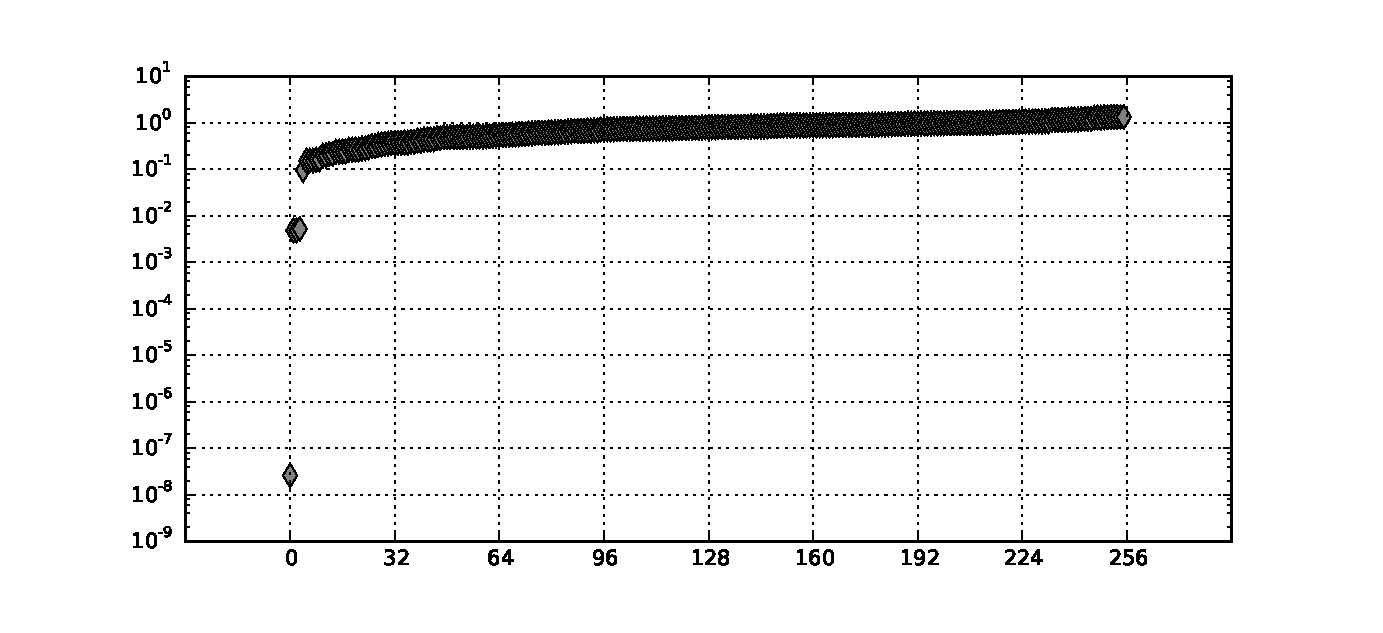
\includegraphics[width=\textwidth]{images/oscvalues.eps}
  \caption{The sorted magnitudes of the oscillatory parts of $\theta\big(
    \boldsymbol{h}_j - \tfrac{1}{2}\Abel_0^{\DivC}, \Omega \big)$ for each of
    the 256 half-lattice vectors $\boldsymbol{h}_j$. Note that the half-lattice
    vector resulting in the correct RCV produces a theta value approximately
    five orders of magnitude closer to zero than the others.}
  \label{fig:oscvalues}
\end{figure}

Even with the default numerical integration and Riemann theta accuracy of
$10^{-8}$ the choice of half-lattice vector producing the above RCV results in a
Riemann theta value that is several orders of magnitude closer to zero than with
the incorrect choices of half-lattice vector, as shown in Figure
\ref{fig:oscvalues}.

Let $\DivD$ be the divisor consisting of the three places lying above $x=2$ each
of multiplicity one. $\DivD$ is an effictive divisor of degree $g-1 = 3$.
Therefore, $\RCV(P_0) + \Abel(P_0,\DivD)$ is also a member of the theta divisor.
\begin{lstlisting}
sage: D = sum(places_above_two)
sage: W = J(AbelMap(D) + K(P0))
sage: v = RiemannTheta.oscillatory_part(W, Omega)
sage: abs(v)
1.09506634962e-10
\end{lstlisting}
\end{example}



%%% Local Variables:
%%% mode: latex
%%% TeX-master: "../thesis"
%%% End:

%%%%%%%%%%%%%%%%%%%%%%%%%%%%%%%%%%%%%%%%%%%%%%%%%%%%%%%%%%%%%%%%%%%%%%%%%%%%%%%
\chapter{Application: Finite-Genus Solutions of the Kadomtsev--Petviashvili
  Equation}\label{ch:kp}
%%%%%%%%%%%%%%%%%%%%%%%%%%%%%%%%%%%%%%%%%%%%%%%%%%%%%%%%%%%%%%%%%%%%%%%%%%%%%%%

The Kadomtsev--Petviashvili (KP) equation is a natural two-dimensional
generalization of the Korteweg de-Vries (KdV) equation describing
two-dimensional shallow water wave propagation.

\begin{figure}
  \centering
  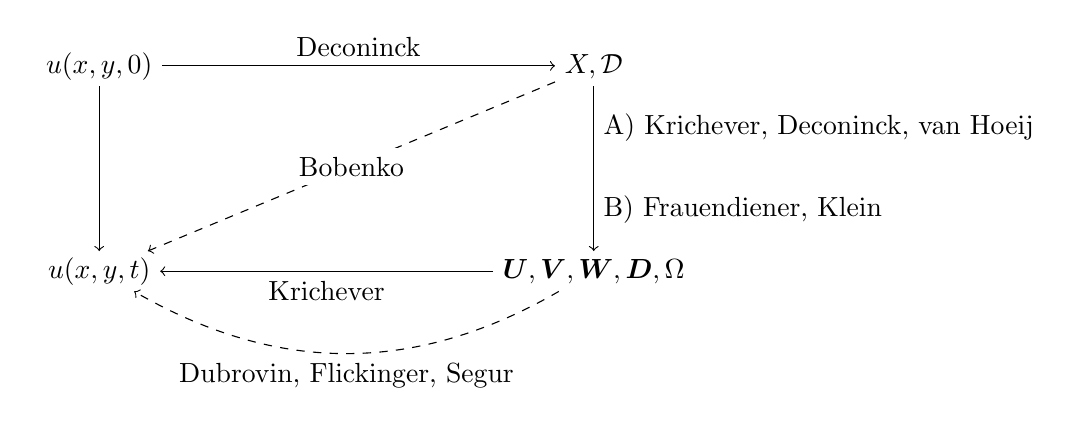
\begin{tikzpicture}[descr/.style={fill=white}]
    \matrix(m)[matrix of math nodes, row sep=6em, column sep=12em, text
    height=1.5ex, text depth=0.25ex] {
      u(x,y,0) & X,\DivD \\
      u(x,y,t) & \boldsymbol{U},\boldsymbol{V},\boldsymbol{W},\boldsymbol{D}, \Omega \\
    };

    \path[->]
      (m-1-1) edge node[auto] {Deconinck} (m-1-2)
      (m-1-1) edge node[auto] {} (m-2-1)
      (m-1-2) edge node[near start,right]
                   {A) Krichever, Deconinck, van Hoeij}
                   node[near end, right]
                   {B) Frauendiener, Klein}
                   (m-2-2)
      (m-1-2) edge[dashed] node[descr] {Bobenko} (m-2-1)
      (m-2-2) edge[bend left,dashed] node[auto]
              {Dubrovin, Flickinger, Segur}
              (m-2-1)
      (m-2-2) edge node[auto] {Krichever} (m-2-1);
  \end{tikzpicture}
  \caption{A map of contributions to the solution to the initial value problem
    for the KP equation. The path taken by this work is represented by the solid
    arrows. Alternate approaches are shown as dashed arrows.}
\end{figure}



Other approaches exist for computing with Riemann surfaces. Bobenko and
collaborators \cite{belokolos, BobenkoBordag89} compute solutions of integrable
equations using a Schottky group representation for the associated surface. To
our knowledge, the only paper dealing with all Riemann surfaces represented by
algebraic curves is by Frauendiener, Klein, and Shramchenko who compute the
homology of a Riemann surface from the monodromy of an underlying algebraic
curve, following \cite{dvh1}. Otherwise, authors have restricted themselves to
specific families of Riemann surfaces such as hyperelliptic ones
\cite{FrauendienerKlein06,FrauendienerKlein15} or low genus ones
\cite{DFS97,FinkelSegur85,DeconinckSwierczewski13}. Our aim throughout is the
development of algorithms capable of dealing with arbitrary compact connected
Riemann surfaces, as is required for the investigation of solutions of, for
instance, the KP equation \cite{DS98,Shiota86}.


%%%%%%%%%%%%%%%%%%%%%%%%%%%%%%%%%%%%%%%%%%%%%%%%%%%%%%%%%%%%%%%%%%%%%%%%%%%%%%%
\section{Finite Genus Solutions}\label{sec:kp-finite-genus-solutions}
%%%%%%%%%%%%%%%%%%%%%%%%%%%%%%%%%%%%%%%%%%%%%%%%%%%%%%%%%%%%%%%%%%%%%%%%%%%%%%%

There is a large class of so-called ``finite-genus'' solutions to the KP
equation. These solutions are quasiperiodic -- functions $f$ such that $f(z + T)
\approx f(z)$ for some quasiperiod $T$ and some meaning of ``approximate''. For
example, a function satisfying $f(z + T) = Cf(z)$ is called geometric
quasiperiodic. Similarly, a function satisfying $f(z + T) = f(z) + C$ is called
arithmetic quasiperiodic. In fact, we have already seen an example of
quasiperiodicity in the Riemann theta function $\theta(z,\Omega)$. The
quasiperiod is $T = m + \Omega n$ for $m,n in \ZZ^g$ and the Riemann theta
function satisfies the functional equation,
\begin{equation}
  \theta(z + m + \Omega n, \Omega)
  =
  e^{-2 \pi i \left( \tfrac{1}{2} n \cdot \Omega n + n \cdot z \right)}
  \theta(z,\Omega).
\end{equation}

In order to define the class of finite-genus solutions to the KP equation we
must first derive some components.

Given a genus $g$ Riemann surface $X$ with normalized basis of holomorphic
one-forms $\mathbf{\omega} = \{ \omega_1, \ldots, \omega_g\}$


\begin{theorem} \label{thm:finite-genus-solutions} The KP equation
\begin{equation} \label{eqn:kp}
  u = c + 2 \partial_x^2 \log \theta\Big( \boldsymbol{U}x +
  \boldsymbol{V}y + \boldsymbol{W}t + \Abel\big(P^\infty,\DivD\big) -
  \RCV(P^\infty), \Omega \Big),
\end{equation}

\end{theorem}


%%%%%%%%%%%%%%%%%%%%%%%%%%%%%%%%%%%%%%%%%%%%%%%%%%%%%%%%%%%%%%%%%%%%%%%%%%%%%%%
\section{Symmetric Period Bases}\label{sec:kp-symmetric-period-bases}
%%%%%%%%%%%%%%%%%%%%%%%%%%%%%%%%%%%%%%%%%%%%%%%%%%%%%%%%%%%%%%%%%%%%%%%%%%%%%%%

% TODO theorem from Belokolos

The approach discussed above provides solutions to the KP equation but make no
restrictions on smoothness. However, for general solutions of the form
\begin{equation} \label{eqn:kp}
  u = c + 2 \partial_x^2 \log \theta\Big(
  \boldsymbol{U}x + \boldsymbol{V}y + \boldsymbol{W}t + \boldsymbol{D},
  \Omega \Big),
\end{equation}
there are certain restrictions imposed on the Riemann surface itself as well as
the choice of phase shift $\boldsymbol{D}$ in order to obtain solutions to the
KP equation that are real and smooth. In this section we will describe a
technique due to Kalla and Klein used to derive such a solution as well as the
algorithmic design in Abelfunctions. Note that this approach makes no direct
contribution to the solution to the initial value problem but is nonetheless an
important perspective of the study of solutions to the KP equation.

%%%%%%%%%%%%%%%%%%%%%%%%%%%%%%% TODO FINISH
We begin with a central theorem.
\begin{theorem} \cite{belokolos1994algebro} For smoothness and reality of
  solutions to the KP equation it is necessary and sufficient that, for a given
  Riemann surface $X$, place at infinity $P_\infty$, and local parameter $p =
  k^{-1}$ at $P_\infty$, that the following conditions are satisfied for the
  vector $\boldsymbol{D}$:
  \begin{itemize}
  \item $X$ admits and antiholomorphic involution $\tau : X \to X, \tau^2 = 1,$
    where $\tau P_\infty = P_\infty$ and $\tau^* k = \bar{k}$.
  \item The set of all fixed ovals of the involution $\tau$ decomposes $X$ into
    two connected components $X^+$ and $X^-$.
  \item If $P_\infty \in $
    
  \end{itemize}

\end{theorem}

The algorithms discussed in Chapter \ref{ch:background} compute the period
matrix of a Riemann surface using the canonical basis of of cycles determined by
the Tretkoff and Tretkoff algorithm \cite{TretkoffTretkoff84}. However, these
cycles may not be invariant under the antiholomorphic involution defined on a
real plane algebraic curve.

\begin{definition} \label{def:topological-type} The {\bf topological} type of a
  real Riemann surface $X$ is given by the tuple $(g, k, a)$ where $g$ is the
  genus of the surface, $k$ is the number of real ovals, and $a = 0$ if the
  curve is dividing and $a = 1$ if the curve is non-dividing. The {\bf real
    ovals} of a surface are the connected components of $X(\mathbb{R})$. $X$ is
  called {\bf dividing} if and only if $X \setminus X(\mathbb{R})$ has two
  connected components. Otherwise, it has one connected component and is called
  {\bf non-dividing}.
\end{definition}

\begin{definition} \label{def:symmetric-homology-basis} Let $\tau$ be an
  antiholomorphic involution on a real Riemann surface $X$. A canonical homology
  basis $(\mathcal{A}, \mathcal{B})$ is called a {\bf symmetric homology basis}
  if it satisfies,
  \begin{equation}
    \begin{pmatrix} \tau \mathcal{A} \\ \tau \mathcal{B} \end{pmatrix}
    =
    \begin{pmatrix}
      \mathbb{I}_g & 0 \\
      \mathbb{H} & -\mathbb{I}_g
    \end{pmatrix}
    \begin{pmatrix} \mathcal{A} \\ \mathcal{B} \end{pmatrix},
  \end{equation}
  where $\mathbb{H}$ is a block diagonal matrix depending on the topological
  type $(g, k, a)$ of $X$ and has one of the following forms:
  \begin{align}
    \mathbb{H} &= \begin{pmatrix}
      0 & 1 &        &   &   &   &        &   \\
      1 & 0 &        &   &   &   &        &   \\
        &   & \ddots &   &   &   &        &   \\
        &   &        & 0 & 1 &   &        &   \\
        &   &        & 1 & 0 &   &        &   \\
        &   &        &   &   & 0 &        &   \\
        &   &        &   &   &   & \ddots &   \\
        &   &        &   &   &   &        & 0
      \end{pmatrix}, & \text{if $k>0$ and $a=0$}, \\
    \mathbb{H} &= \begin{pmatrix}
      \mathbb{I}_{g+1-k} & \\
      & 0
    \end{pmatrix},  & \text{if $k>0$ and $a=1$}, \\
    \mathbb{H} &= \begin{pmatrix}
      0 & 1 &        &   &   \\
      1 & 0 &        &   &   \\
        &   & \ddots &   &   \\
        &   &        & 0 & 1 \\
        &   &        & 1 & 0
      \end{pmatrix}, & \text{if $k=0$ and $g$ is even}, \\
    \mathbb{H} &= \begin{pmatrix}
      0 & 1 &        &   &   &   \\
      1 & 0 &        &   &   &   \\
        &   & \ddots &   &   &   \\
        &   &        & 0 & 1 &   \\
        &   &        & 1 & 0 &   \\
        &   &        &   &   & 0
    \end{pmatrix}, & \text{if $k=0$ and $g$ is odd}.
  \end{align}
\end{definition}

%%%%%%%%%% TODO DISCUSSION OF SYMPLECTIC TRANSFORMATIONS ON HOMOLOGY BASES
%%%%%%%%%% cf. p30 of belokolos
Recall that 

The goal is to construct a symplectic transformation
\begin{equation}
  \Gamma = \begin{pmatrix} A & B \\ C & D \end{pmatrix}
\end{equation}
mapping an arbitrary canonical homology basis $(\tilde{\mathcal{A}},
\tilde{\mathcal{B}})$ to an equivalent, in the sense of Siegel, symmetric
homology basis $(\mathcal{A}, \mathcal{B})$ satisfying,
\begin{equation}
  \begin{pmatrix} \tau \mathcal{A} \\ \tau \mathcal{B} \end{pmatrix}
  \begin{pmatrix}
      \mathbb{I}_g & 0 \\
      \mathbb{H} & -\mathbb{I}_g
  \end{pmatrix}
  \begin{pmatrix} \mathcal{A} \\ \mathcal{B} \end{pmatrix},
\end{equation}
and, therefore, the necessary and sufficient conditions to produce real and
smooth solutions to the KP equation. Vinnikov proves \cite{vinnikov1993self}
that such a symplectic transformation exists,
\begin{equation}
  \begin{pmatrix} A & B \\ C & D \end{pmatrix}
  \begin{pmatrix} \tau{\mathcal{A}} \\ \tau{\mathcal{B}} \end{pmatrix} = 
  \begin{pmatrix} \mathcal{A} \\ \mathcal{B} \end{pmatrix}.
\end{equation}

We summarize the work of Kalla and Klein

%%%%%%%%%%%%%%%%%%%%%%%%%%%%%%%%%%%%%%%%%%%%%%%%%%%%%%%%%%%%%%%%%%%%%%%%%%%%%%%
\section{Computations and Results}\label{sec:kp-computations-and-results}
%%%%%%%%%%%%%%%%%%%%%%%%%%%%%%%%%%%%%%%%%%%%%%%%%%%%%%%%%%%%%%%%%%%%%%%%%%%%%%%

%%%%%%%%%%%%%%%%%%%%%%%%%%%%%%%%%%%%%%%%%%%%%%%%%%%%%%%%%%%%%%%%%%%%%%%%%%%%%%%
\section{Future Work}\label{sec:kp-future-work}
%%%%%%%%%%%%%%%%%%%%%%%%%%%%%%%%%%%%%%%%%%%%%%%%%%%%%%%%%%%%%%%%%%%%%%%%%%%%%%%
%%%%%%%%%%%%%%%%%%%%%%%%%%%%%%%%%%%%%%%%%%%%%%%%%%%%%%%%%%%%%%%%%%%%%%%%%%%%%%%
\chapter{Application: Determinantal Representations of Algebraic
  Curves}\label{ch:determinantal}
%%%%%%%%%%%%%%%%%%%%%%%%%%%%%%%%%%%%%%%%%%%%%%%%%%%%%%%%%%%%%%%%%%%%%%%%%%%%%%%

%%%%%%%%%%%%%%%%%%%%%%%%%%%%%%%%%%%%%%%%%%%%%%%%%%%%%%%%%%%%%%%%%%%%%%%%%%%%%%%
\section{Background}\label{sec:determinantal-introduction}
%%%%%%%%%%%%%%%%%%%%%%%%%%%%%%%%%%%%%%%%%%%%%%%%%%%%%%%%%%%%%%%%%%%%%%%%%%%%%%%

%%%%%%%%%%%%%%%%%%%%%%%%%%%%%%%%%%%%%%%%%%%%%%%%%%%%%%%%%%%%%%%%%%%%%%%%%%%%%%%
\section{Computations and
  Results}\label{sec:determinantal-computation-and-results}
%%%%%%%%%%%%%%%%%%%%%%%%%%%%%%%%%%%%%%%%%%%%%%%%%%%%%%%%%%%%%%%%%%%%%%%%%%%%%%%

%%%%%%%%%%%%%%%%%%%%%%%%%%%%%%%%%%%%%%%%%%%%%%%%%%%%%%%%%%%%%%%%%%%%%%%%%%%%%%%
\section{Future Work}\label{sec:determinantal-future-work}
%%%%%%%%%%%%%%%%%%%%%%%%%%%%%%%%%%%%%%%%%%%%%%%%%%%%%%%%%%%%%%%%%%%%%%%%%%%%%%%

% bibliography
%
\bibliographystyle{plain}
\bibliography{thesis}

% appendices
%
\appendix
\include{chapters/appendix}


\end{document}
%%% Local Variables:
%%% mode: latex
%%% TeX-master: t
%%% End:
